\documentclass[11pt,a4paper]{article}
\usepackage[margin=2.2cm]{geometry}
\usepackage{graphicx}
\usepackage{amsmath,amssymb}
\usepackage{booktabs}
\usepackage{longtable}
\usepackage[colorlinks=true,linkcolor=black,urlcolor=blue,citecolor=black]{hyperref}
\usepackage{caption}
\usepackage{tikz}
\usetikzlibrary{positioning,fit,arrows.meta,shapes.geometric,backgrounds,calc}
\captionsetup{font=small,labelfont=bf}
\graphicspath{{../Plot/}}
\setlength{\parskip}{0.4em}
\setlength{\parindent}{0pt}

\tikzset{
  latent/.style={circle,draw,thick,minimum size=11mm,inner sep=0pt,font=\small},
  obs/.style={latent,fill=gray!25},
  det/.style={circle,draw,thick,double,double distance=1.2pt,minimum size=11mm,inner sep=0pt,
              font=\small},
  dec/.style={rectangle,draw,thick,minimum size=10mm,inner sep=1pt,font=\small},
  fitted/.style={diamond,draw,thick,minimum size=12mm,inner sep=0pt,font=\small},
  fixed/.style={circle,fill=black,minimum size=4pt,inner sep=0pt},
  flabel/.style={font=\scriptsize,align=center},
  edge/.style={-{Latex[length=2mm]},thick},
  fitedge/.style={-{Latex[length=2mm]},thick,dashed},
  plate/.style={draw,rounded corners=6pt,inner sep=7pt,thick,gray},
}

\title{\bfseries HWO ExoEarth Yields for a Mass-Selected Planet Sample\\
in a Narrowed Habitable Zone\\[0.3em]
\large A rederivation of the AYO yield model of Stark et al., laid out as a probabilistic model}
\author{Prepared in the \texttt{yields} vaibify project}
\date{\today}

\begin{document}
\maketitle

\begin{abstract}
\noindent
We ask how many exoEarth candidates the baseline Habitable Worlds Observatory (HWO) mission of
Stark et al.\ (2024) would find if the target population were planets of $0.5$--$2\,M_\oplus$
(with $R = M^{0.27}$) in a habitable zone of $0.96$--$1.20$~AU scaled by $\sqrt{L_\star}$, rather
than the canonical $R \le 1.4\,R_\oplus$ planets in $0.95$--$1.67$~AU. Answering it requires
re-running the survey optimization, because the survey reallocates its time as the expected
number of detections changes. We rederive the Altruistic Yield Optimization (AYO) model from the
published equations and parameters, and write it down as a probabilistic graphical model whose
single decision node is the survey allocation. With the extended-source throughput $T_{\rm sky}$
treated as a function of separation, as Stark et al.\ (2019) define it, the model reproduces
Stark's published 22.5 candidates to 0.5\% with no fitted parameter; the one
throughput factor it carries, previously 1.62, is now $\kappa = 0.988$. Exozodi is a random
variable of the pipeline, marginalized over 200 draws with the survey re-optimized for each.
The model gives a median canonical yield of 19.3 (90\% interval 5.9--51.6)
and a median redefined yield of 4.6 (1.3--15.5).
The yield ratio is $0.245^{+0.035}_{-0.025}$, larger than the occurrence ratio
of $0.204$ because the redefined box removes the faintest planets. The probability of
reaching 25 candidates falls from 35.7\% to 1.19\%. Of 23 independent checks
against the published record, 19 agree, and nine of Stark's figures are reproduced in
their own axes beside the originals. The main remaining disagreement is that this model's
spectral characterization times depend on target difficulty and aperture more steeply than
Stark's. A per-star table gives every target's Earth zone and classic habitable zone and what the
survey expects to find in each.
\end{abstract}

\tableofcontents

%======================================================================
\section{The question and the answer}
\label{sec:answer}

The request was to trace the ExoVista/AYO yield chain back to its assumptions about the planet
population, couple it to a Bayesian sampler, and predict how many planets of
$0.5$--$2\,M_\oplus$, $R = M^{0.27}$, around FGK stars, the baseline HWO mission would find if the
habitable zone were $0.96$--$1.20$~AU for the Sun, scaled as $\sqrt{L_\star}$ for other stars.
The answer is summarized in Table~\ref{tab:answer}.

\begin{table}[htbp]
\centering
\small
\begin{tabular}{lrr}
\toprule
& \textbf{Canonical box} & \textbf{Redefined box} \\
\midrule
Habitable zone (AU, scaled by $\sqrt{L_\star}$) & 0.95--1.67 & 0.96--1.20 \\
Planet selection & $0.8\,(a/\mathrm{EEID})^{-1/2} < R/R_\oplus \le 1.4$ & $0.5 \le M/M_\oplus \le 2$, $R=M^{0.27}$ \\
Occurrence $\eta$ (median, 68\%) & $0.255^{+0.282}_{-0.134}$ & $0.0520^{+0.0577}_{-0.0274}$ \\
Realized yield, median & 19.3 & 4.6 \\
Realized yield, mean & 22.5 & 6.0 \\
Realized yield, 90\% interval & 5.9--51.6 & 1.3--15.5 \\
$P(\ge 25$ candidates$)$ & 35.7\% & 1.19\% \\
\midrule
Occurrence ratio, redefined/canonical & \multicolumn{2}{c}{$0.204^{+0.017}_{-0.016}$} \\
\textbf{Yield ratio, redefined/canonical} & \multicolumn{2}{c}{$\mathbf{0.245^{+0.035}_{-0.025}}$} \\
\bottomrule
\end{tabular}
\caption{The answer for the baseline 6\,m (inscribed) LUVOIR-B-like design. Yields are realized
counts, marginalized over the $\eta_\oplus$ uncertainty, the planet draw, the geometric albedo and
the survey's re-optimization; they are the quantity Stark et al.\ (2024) plot in Fig.~10 and
compute $P_{25}$ from.}
\label{tab:answer}
\end{table}

The yield ratio is the robust result. It is taken at one aperture, inside one implementation,
with the same calibration in numerator and denominator. Across the model revisions of the final
sessions (exozodi, $\eta_\oplus$ width, the separation-dependent $T_{\rm sky}$, and exozodi
marginalized over draws) it has moved only from 0.246 to 0.241 to 0.245, inside its own error
bar. The absolute yields are conditional on the open problem of Sec.~\ref{sec:open}.

Why the yield ratio exceeds the occurrence ratio (Sec.~\ref{sec:ratio}) is itself a result: the
redefined box keeps the brighter, closer-in planets, frees characterization time, and loses some
distant stars, and the first two effects win. A rescaling of Stark's yield by the occurrence ratio
alone would have been wrong by 20\%, in a direction that cannot be predicted without running the
optimization.

%======================================================================
\section{The model as a probabilistic graphical model}
\label{sec:pgm}

\subsection{Why a graphical model}

The AYO yield calculation is usually described procedurally: compute completeness, optimize
exposure times, count planets, then add uncertainty sources one at a time. That description hides
the structure that decides every number in this report --- which quantities are \emph{random},
which are \emph{fixed}, which are \emph{fitted}, and, crucially, which random quantities the
survey planner is allowed to see when it allocates its time. Stark et al.\ (2024, Sec.~3) call
the last distinction \emph{actionable} versus \emph{static} uncertainty. In a graphical model it
has a precise meaning, and it is the single most consequential modelling choice after the
radiometry.

Figure~\ref{fig:pgm} shows the model as an influence diagram: a directed acyclic graph of random
variables with one \emph{decision} node, the survey allocation. Every node is implemented by a
named function in the pipeline, listed in Table~\ref{tab:nodes}.

\begin{figure}[p]
\centering
\resizebox{\textwidth}{!}{%
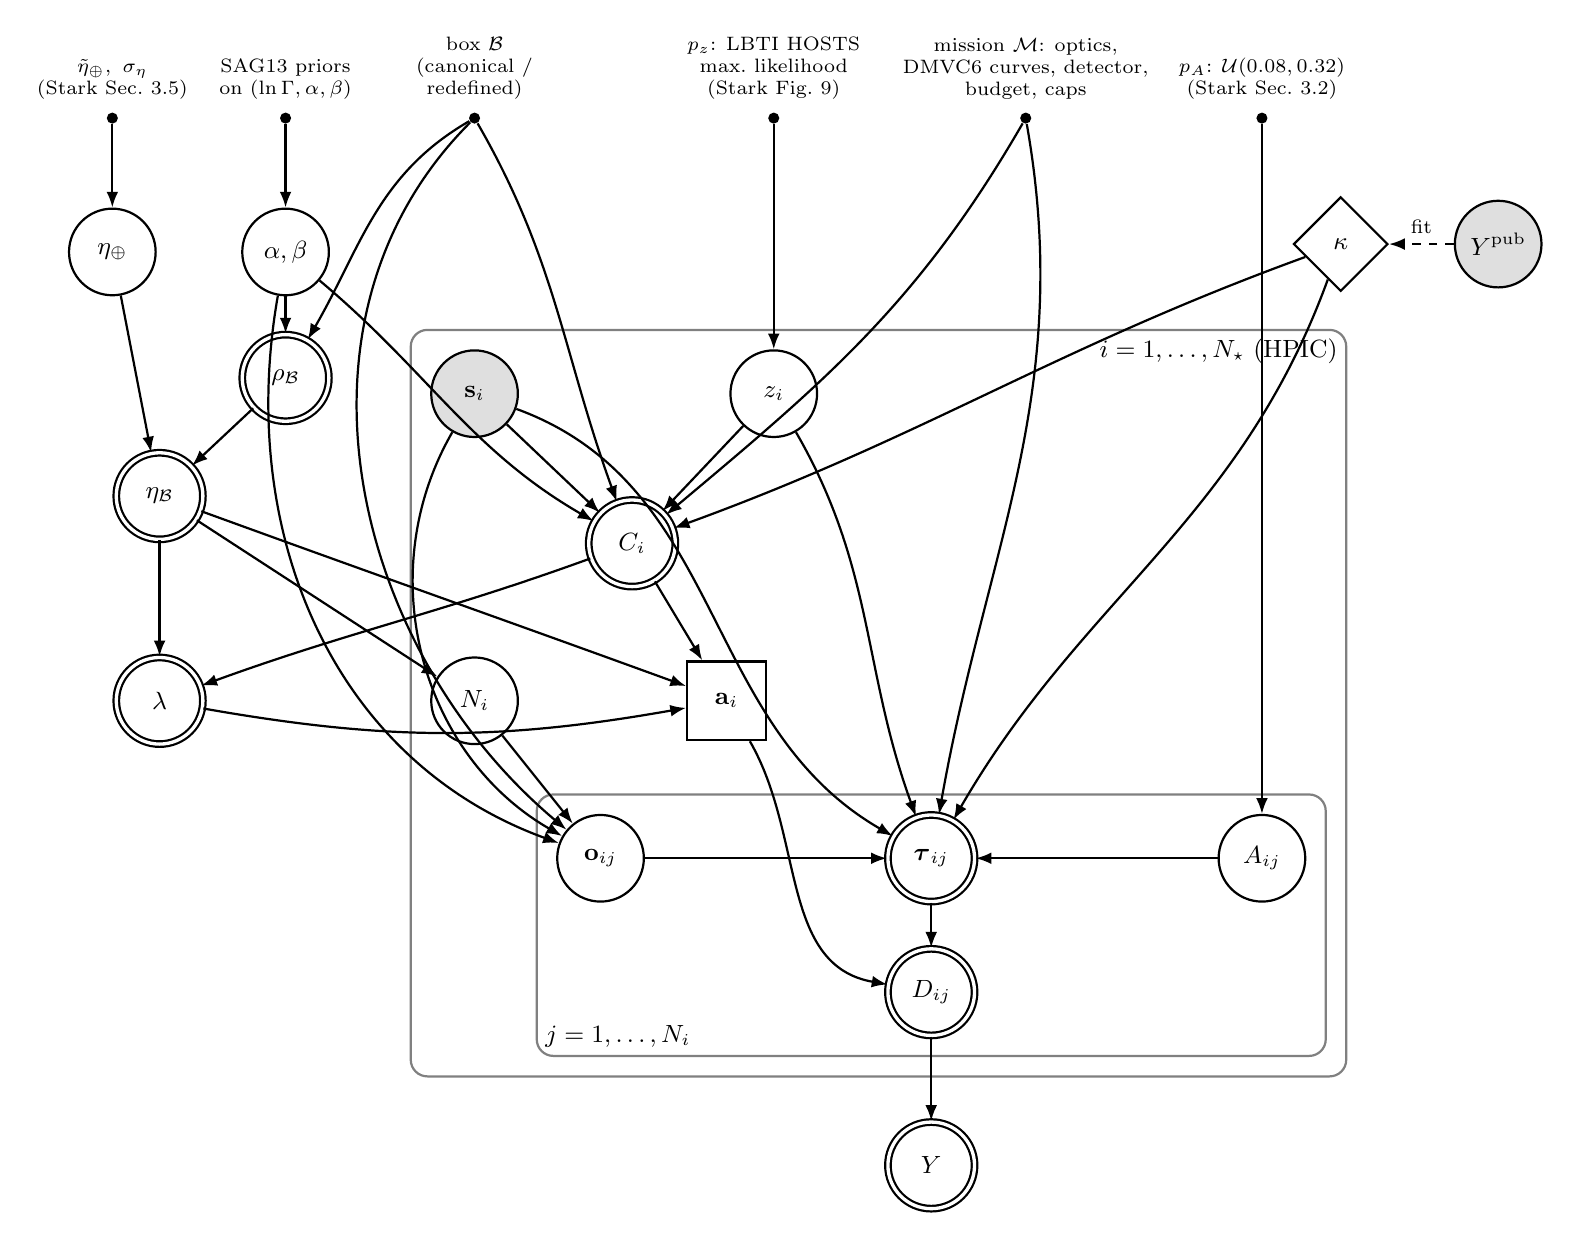
\begin{tikzpicture}[x=1cm,y=1cm]
  % ---- global hyperparameters (fixed) ----
  \node[fixed] (hEta) at (0,0) {};
  \node[flabel,above=1pt of hEta] {$\tilde\eta_\oplus,\ \sigma_\eta$\\(Stark Sec.~3.5)};
  \node[fixed] (hShape) at (2.2,0) {};
  \node[flabel,above=1pt of hShape] {SAG13 priors\\on $(\ln\Gamma,\alpha,\beta)$};
  \node[fixed] (hBox) at (4.6,0) {};
  \node[flabel,above=1pt of hBox] {box $\mathcal{B}$\\(canonical /\\redefined)};
  \node[fixed] (hZ) at (8.4,0) {};
  \node[flabel,above=1pt of hZ] {$p_z$: LBTI HOSTS\\max.\ likelihood\\(Stark Fig.~9)};
  \node[fixed] (hM) at (11.6,0) {};
  \node[flabel,above=1pt of hM] {mission $\mathcal{M}$: optics,\\DMVC6 curves, detector,\\budget, caps};
  \node[fixed] (hA) at (14.6,0) {};
  \node[flabel,above=1pt of hA] {$p_A$: $\mathcal{U}(0.08,0.32)$\\(Stark Sec.~3.2)};
  % ---- global latent / deterministic ----
  \node[latent] (eta) at (0,-1.7) {$\eta_\oplus$};
  \node[latent] (shape) at (2.2,-1.7) {$\alpha,\beta$};
  \node[det] (rho) at (2.2,-3.3) {$\rho_{\mathcal{B}}$};
  \node[det] (etaB) at (0.6,-4.8) {$\eta_{\mathcal{B}}$};
  \node[det] (lambda) at (0.6,-7.4) {$\lambda$};
  \node[fitted] (kappa) at (15.6,-1.6) {$\kappa$};
  \node[obs] (ypub) at (17.6,-1.6) {$Y^{\rm pub}$};
  % ---- star plate ----
  \node[obs] (s) at (4.6,-3.5) {$\mathbf{s}_i$};
  \node[latent] (z) at (8.4,-3.5) {$z_i$};
  \node[det] (C) at (6.6,-5.4) {$C_i$};
  \node[latent] (N) at (4.6,-7.4) {$N_i$};
  \node[dec] (a) at (7.8,-7.4) {$\mathbf{a}_i$};
  % ---- planet plate ----
  \node[latent] (o) at (6.2,-9.4) {$\mathbf{o}_{ij}$};
  \node[det] (tau) at (10.4,-9.4) {$\boldsymbol{\tau}_{ij}$};
  \node[latent] (A) at (14.6,-9.4) {$A_{ij}$};
  \node[det] (D) at (10.4,-11.1) {$D_{ij}$};
  % ---- yield ----
  \node[det] (Y) at (10.4,-13.3) {$Y$};
  \coordinate (Aright) at (15.4,-9.4);
  % ---- plates ----
  \begin{scope}[on background layer]
    \node[plate,fit=(o) (tau) (A) (D)] (pp) {};
    \node[plate,fit=(s) (z) (C) (N) (a) (pp) (Aright)] (sp) {};
  \end{scope}
  \node[font=\small,anchor=south west] at (pp.south west) {$j = 1,\dots,N_i$};
  \node[font=\small,anchor=north east] at (sp.north east) {$i = 1,\dots,N_\star$ (HPIC)};
  % ---- edges ----
  \draw[edge] (hEta) -- (eta);
  \draw[edge] (hShape) -- (shape);
  \draw[edge] (shape) -- (rho);
  \draw[edge] (hBox) to[out=-150,in=60] (rho);
  \draw[edge] (eta) -- (etaB);
  \draw[edge] (rho) -- (etaB);
  \draw[edge] (etaB) -- (lambda);
  \draw[edge] (etaB) to[out=-20,in=160] (a);
  \draw[edge] (etaB) -- (N);
  \draw[edge] (C) to[out=-160,in=20] (lambda);
  \draw[edge] (lambda) to[out=-10,in=-170] (a);
  \draw[edge] (C) -- (a);
  \draw[edge] (hZ) -- (z);
  \draw[edge] (s) -- (C);
  \draw[edge] (z) -- (C);
  \draw[edge] (hBox) to[out=-135,in=140] (o);
  \draw[edge] (s) to[out=-20,in=150] (tau);
  \draw[edge] (hBox) to[out=-60,in=110] (C);
  \draw[edge] (shape) to[out=-40,in=150] (C);
  \draw[edge] (hM) to[out=-120,in=40] (C);
  \draw[edge] (kappa) to[out=-160,in=20] (C);
  \draw[edge] (s) to[out=-120,in=150] (o);
  \draw[edge] (shape) to[out=-100,in=160] (o);
  \draw[edge] (N) -- (o);
  \draw[edge] (o) -- (tau);
  \draw[edge] (A) -- (tau);
  \draw[edge] (hA) -- (A);
  \draw[edge] (z) to[out=-60,in=110] (tau);
  \draw[edge] (hM) to[out=-80,in=80] (tau);
  \draw[edge] (kappa) to[out=-110,in=60] (tau);
  \draw[edge] (tau) -- (D);
  \draw[edge] (a) to[out=-60,in=170] (D);
  \draw[edge] (D) -- (Y);
  \draw[fitedge] (ypub) -- node[above,font=\scriptsize]{fit} (kappa);\end{tikzpicture}}

\vspace{0.6em}
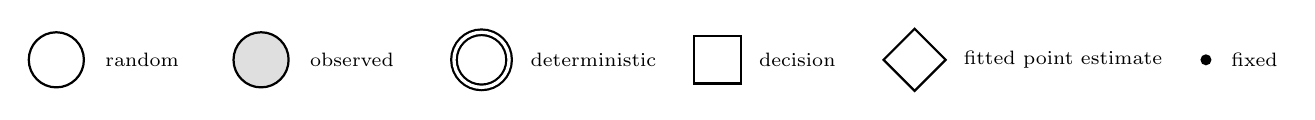
\begin{tikzpicture}[x=1cm,y=1cm]
  \node[latent,minimum size=7mm] at (0,0) {}; \node[font=\scriptsize,anchor=west] at (0.5,0) {random};
  \node[obs,minimum size=7mm] at (2.6,0) {}; \node[font=\scriptsize,anchor=west] at (3.1,0) {observed};
  \node[det,minimum size=7mm] at (5.4,0) {}; \node[font=\scriptsize,anchor=west] at (5.9,0) {deterministic};
  \node[dec,minimum size=6mm] at (8.4,0) {}; \node[font=\scriptsize,anchor=west] at (8.8,0) {decision};
  \node[fitted,minimum size=8mm] at (10.9,0) {}; \node[font=\scriptsize,anchor=west] at (11.4,0) {fitted point estimate};
  \node[fixed] at (14.6,0) {}; \node[font=\scriptsize,anchor=west] at (14.8,0) {fixed};
\end{tikzpicture}
\caption{The yield model as an influence diagram. Outer plate: the $N_\star$ screened HPIC stars;
inner plate: the $N_i$ planets actually present around star $i$. The survey allocation
$\mathbf{a}_i = (\tau_i, k_i)$ --- exposure per visit and number of visits --- is the one decision
node; it is set by the equal-slope multiplier $\lambda$ from the planner's completeness curves
$C_i$ and the box occurrence rate $\eta_{\mathcal{B}}$. A planet is counted ($D_{ij} = 1$) when
its detection time at some visit is within the allocation and its spectral characterization time
is within the two-month cap; $Y = \sum_{ij} D_{ij}$. The throughput factor $\kappa$ is not a random
variable: it is fitted once, at fixed exozodi, to the published expected yield $Y^{\rm pub} = 22.5$
(dashed), and comes out at 0.988, so the edge carries almost no information. Four stars with LBTI-measured exozodi have $z_i$ observed rather than drawn (not shown).
The edges that decide the uncertainty budget are the ones \emph{into} $\mathbf{a}_i$: $\eta_\oplus$
and $z_i$ reach it (actionable), $A_{ij}$ and $N_i$ do not (static).}
\label{fig:pgm}
\end{figure}

\subsection{The nodes}

\begin{table}[htbp]
\centering
\scriptsize
\begin{tabular}{p{1.2cm}p{3.2cm}p{5.6cm}p{3.6cm}}
\toprule
\textbf{Node} & \textbf{Type} & \textbf{Specification} & \textbf{Source; step} \\
\midrule
$\eta_\oplus$ & random, global & lognormal, median 0.257, $\ln$-width 0.76 (Sec.~\ref{sec:eta}) & Stark+2024 Sec.~3.5, read at $z=1$; A06 \\
$\alpha,\beta$ & random, global & SAG13 shape; posterior of an \texttt{emcee} chain, used only through $\rho_\mathcal{B}$ & SAG13; A06 \\
$\rho_\mathcal{B}$ & deterministic & $\eta_\mathcal{B}/\eta_\oplus$, the SAG13 integral over $\mathcal{B}$ relative to the canonical box; independent of $\Gamma$ & A06 \\
$\eta_\mathcal{B}$ & deterministic & $\eta_\oplus\,\rho_\mathcal{B}$ & A06 \\
$\mathbf{s}_i$ & observed & $d$, $L_\star$, $T_{\rm eff}$, $R_\star$, HIP id & HPIC (Tuchow+2024); A01 \\
$z_i$ & random, per star & exozodi level, $z_i \sim p_z$; four stars fixed at LBTI values; 200 joint draws of $\mathbf{z}$ & Stark+2024 Sec.~3.3, Fig.~9; A02, A04 \\
$C_i$ & deterministic & planner's completeness $C_i(\tau, k)$ at $A_G = 0.2$, over exposure and visits, counting only planets that are also characterizable & Stark+2019; A04 \\
$\lambda$ & deterministic & equal-slope multiplier closing the two-year budget & Stark+2014; A05 \\
$\mathbf{a}_i$ & decision & $(\tau_i, k_i)$: the vertex of star $i$'s concave cost envelope at slope $\lambda$ & A05, A07 \\
$N_i$ & random, per star & $N_i \sim \mathrm{Poisson}(\eta_\mathcal{B})$ & Stark+2024 Sec.~3.1; A07 \\
$\mathbf{o}_{ij}$ & random, per planet & circular orbit: $a$, $R$ from SAG13 over $\mathcal{B}$; $\cos i \sim \mathcal{U}$; independent epoch per visit & ExoVista/AYO; A04 \\
$A_{ij}$ & random, per planet & geometric albedo, $\mathcal{U}(0.08, 0.32)$ & Stark+2024 Sec.~3.2; A04 \\
$\boldsymbol{\tau}_{ij}$ & deterministic & detection time per visit (two channels in quadrature, S/N 7) and characterization time (R 140, best of nine bandpasses, best orbital phase) & Stark+2019 Eqs.~1--9; A04 \\
$D_{ij}$ & deterministic & $\mathbb{1}[\min_{v \le k_i}\tau^{\rm det}_{ijv} \le \tau_i \ \wedge\ \tau^{\rm char}_{ij} \le 2\,\mathrm{mo}]$ & Stark+2019 Sec.~3; A04 \\
$Y$ & deterministic & $\sum_{i,j} D_{ij}$ & A07 \\
$\kappa$ & fitted & throughput factor on every band, fitted to $Y^{\rm pub}$: 0.988 & A03 \\
\bottomrule
\end{tabular}
\caption{Every node of Fig.~\ref{fig:pgm}, what it is, and where it comes from.}
\label{tab:nodes}
\end{table}

\subsection{The joint distribution, and how the pipeline marginalizes it}
\label{sec:joint}

Conditioning on the fixed quantities $(\mathcal{M}, \mathcal{B}, \kappa, \{\mathbf{s}_i\})$, the
graph factorizes as
\begin{multline}
p(\eta_\oplus, \alpha, \beta, \mathbf{z}, \mathbf{N}, \mathbf{o}, \mathbf{A}, Y)
= p(\eta_\oplus)\,p(\alpha,\beta)\prod_{i} p_z(z_i)\,
\mathrm{Poisson}\!\left(N_i;\ \eta_\mathcal{B}\right) \\
\times \prod_{j=1}^{N_i} p(\mathbf{o}_{ij} \mid \alpha, \beta, \mathcal{B}, \mathbf{s}_i)\,p_A(A_{ij})
\cdot \delta\!\Big(Y - \sum_{ij} D_{ij}\Big),
\label{eq:joint}
\end{multline}
with the allocation entering through $D_{ij}$ as the deterministic function
\begin{equation}
\mathbf{a}_i = \mathbf{a}_i\!\left(\lambda(\eta_\mathcal{B}, \mathbf{C}),\ C_i\right),
\qquad C_i = C_i(\mathbf{s}_i, z_i, \mathcal{M}, \kappa, \mathcal{B}, \alpha, \beta).
\label{eq:alloc}
\end{equation}

Two properties make this tractable, and the pipeline uses both.

\textbf{Poisson thinning.} Given the allocation, planets are counted independently with a
probability that depends only on the star. Marginalizing the planet draw inside the plate is then
exact: if $N_i \sim \mathrm{Poisson}(\eta_\mathcal{B})$ and each planet is counted with
probability $\bar{C}_i$ --- the completeness at the allocated vertex, averaged over the albedo
draw --- the counted planets are $\mathrm{Poisson}(\eta_\mathcal{B}\bar{C}_i)$, and the survey
total is
\begin{equation}
Y \mid \eta_\oplus, \mathbf{z} \ \sim\ \mathrm{Poisson}\!\Big(\Lambda(\eta_\oplus, \mathbf{z})\Big),
\qquad
\Lambda = \eta_\mathcal{B} \sum_i \bar{C}_i\!\left(\mathbf{a}_i(\eta_\mathcal{B}, \mathbf{z})\right).
\label{eq:thinning}
\end{equation}
Step A07 evaluates $\Lambda$ on a 24-node grid in $\eta_\oplus$, \emph{re-optimizing the survey
at every node}, interpolates it, and draws one Poisson count per posterior sample of
$\eta_\oplus$ (14,400 samples). This is Stark's construction exactly: his Sec.~3.1 draws
a Poisson number of planets per star and counts those with a valid visit record.

\textbf{Albedo is static, so it enters $\bar{C}_i$ and not $\mathbf{a}_i$.} The planner allocates
against $C_i$ computed at $A_G = 0.2$; the count is then read from the same planets and orbits
with $A_{ij}$ drawn. A darker-than-planned planet can fail the fixed allocation; a brighter one
gains little. This asymmetry is the whole of the albedo penalty, and the graph makes it
unavoidable: $A_{ij}$ has no path into $\mathbf{a}_i$.

\textbf{What is marginalized, and what is not yet.}
\begin{itemize}
\item $\eta_\oplus$: marginalized, with the survey re-optimized per value (actionable).
\item $N_i$, $\mathbf{o}_{ij}$, $A_{ij}$: marginalized exactly by thinning, Eq.~\eqref{eq:thinning}.
\item $\alpha, \beta$: marginalized for the \emph{ratio} $\rho_\mathcal{B}$; the planet
population inside each box uses the SAG13 central values.
\item $\mathbf{z}$: marginalized over 200 joint draws (Stark uses 500), with the survey
\emph{re-optimized for every draw}, because exozodi is actionable. A04 tabulates each star's
completeness on a 23-level exozodi grid (0--1024 zodis) and each draw interpolates between levels;
against direct evaluation at the drawn levels this changes the optimized yield by at most
0.24\%. Each posterior sample of $\eta_\oplus$ is paired with one draw of $\mathbf{z}$.
Over the draws the fixed-$\eta_\oplus$ yield is 18.30 with a draw-to-draw scatter of
0.57.
\end{itemize}

\subsection{Actionable and static, stated precisely}

A source of uncertainty is \emph{actionable} if its node has a directed path into the decision
node, and \emph{static} if it does not. In Fig.~\ref{fig:pgm}:
\begin{itemize}
\item $\eta_\oplus \to \eta_\mathcal{B} \to \lambda \to \mathbf{a}_i$: actionable. A mission that
finds more planets must spend more time characterizing them, so the survey that maximizes yield
depends on $\eta_\oplus$. This is why yield is sub-linear in $\eta_\oplus$ and why the
redefined yield cannot be obtained by rescaling.
\item $z_i \to C_i \to \mathbf{a}_i$: actionable. Exozodi is measured on the first visit and the
survey adapts (Stark et al.\ 2015).
\item $A_{ij}$, $N_i$, $\mathbf{o}_{ij}$: static. The planner cannot know which stars host
planets, where they are, or how dark they are.
\end{itemize}
Every observational bias in this problem --- the albedo penalty, the exozodi penalty, the
difference between Stark's red and purple curves --- is a statement about which of these paths
exist. Getting a path wrong changes a penalty by a factor of several, as Appendix~\ref{app:ledger}
records.

%======================================================================
\section{The nodes, specified}
\label{sec:nodes}

\subsection{Stars: HPIC}

The target list is the HWO Preliminary Input Catalog (Tuchow et al.\ 2024), the list Stark et al.\
(2024) state they use: 11,757 dwarfs within 50\,pc, 7,767 of them FGK. Stellar photon
fluxes come from a blackbody at the catalogued $T_{\rm eff}$ and $R_\star$; against HPIC's measured
$V$ for 674 stars the median residual is +0.019\,mag over 5300--7300\,K, and the same
fluxes agree with EXOSIMS's Pickles templates to 0.979. The survey pool is the 1,500 stars
with the widest habitable zones in $\lambda/D$ after a box-aware noise-floor screen.

\subsection{Occurrence: $\eta_\oplus$, and why its width is read as one sigma}
\label{sec:eta}

Stark et al.\ (2024) Sec.~3.5 derive $\eta_\oplus$ by integrating the Bryson et al.\ (2021) Kepler
DR25 posteriors over their canonical domain, drawing equally from Bryson's two bounding
completeness-extrapolation cases, and quote $0.26^{+0.29}_{-0.14}$ as a mean with an 86\% interval.
Bryson's posterior chains are not published: the paper's repository omits the output directories
that hold them, and the author's site holds only the completeness contours. The distribution must
therefore be reconstructed, and the choice is decided by Stark's own Fig.~10.

Holding this model's yield-versus-$\eta_\oplus$ curve at Stark's fixed-$\eta_\oplus$ level (his
red curve, mean 17.35), the lognormal $\eta_\oplus$ that turns his red curve into his
purple curve has median 0.26 and $\ln$-width 0.80, reproducing the purple curve
to a total-variation distance of 0.019. Reading the quoted interval as 86\%, as the text
labels it, gives a $\ln$-width of 0.52, a distance of 0.142, and a peak at
15 against the published 10. Reading it as a one-sigma (68\%) interval
gives $\ln$-width 0.76, a distance of 0.024, and a peak at 12. Bryson's
Fig.~14, digitized from its vector source, shows each extrapolation case with a $\ln$-width of about
0.8, consistent with the figure and not with the 86\% reading. This model therefore reads the
interval at $z = 1$ (Table~\ref{tab:nodes}), giving a mean of 0.343; the text's
reading remains available as a command-line option.

The redefined box enters only through $\rho_\mathcal{B}$, the ratio of SAG13 integrals, which does
not depend on the normalization $\Gamma$. Its posterior comes from an \texttt{emcee} chain over
$(\ln\Gamma, \alpha, \beta)$ with SAG13 priors, and is narrow because $\Gamma$ cancels.

\subsection{Exozodi: the HOSTS distribution and four measured stars}
\label{sec:exozodi}

Each star's exozodi level is drawn from the LBTI HOSTS maximum-likelihood distribution that
Stark et al.\ (2024) use, digitized from the vector content stream of their Fig.~9 (red): a median
of 2.98 zodis, against Stark's stated three, with 21\% of draws above 100
zodis. The histogram carries 0.948 of the implied $10^4 \times 500$ draws; the shortfall is
renormalized rather than placed off-axis, because doing so is what reproduces the stated median.
$\epsilon$~Eri (297 zodis), $\theta$~Boo (148), 72~Her (588; ``w~Her'' in HPIC) and 110~Her (235)
are pinned to their LBTI measurements, as Stark does, whenever levels are drawn.

The heavy tail matters more than the median. A star at hundreds of zodis is effectively removed
from the survey; the lognormal stand-in this replaced put 0.2\% of stars above 100 zodis and gave
an exozodi penalty of 0.7\%, against Stark's 11\%. The exozodi surface brightness follows Stark
(2014) App.~C: a constant habitable-zone optical depth, evaluated at the EEID, with solar colours.

\subsection{Radiometry and exposure times: $\boldsymbol{\tau}_{ij}$}

Exposure times follow Stark et al.\ (2019) Eq.~1,
\begin{equation}
\tau = (\mathrm{S/N})^2\,\frac{\mathrm{CR_p} + 2\,\mathrm{CR_b}}{\mathrm{CR_p}^2},
\end{equation}
with backgrounds from leaked starlight, local zodi, exozodi and the detector (dark current and
clock-induced charge with the $6.73$ Geiger factor of Stark 2019 Eq.~9). The zodiacal and
exozodiacal backgrounds carry the extended-source throughput $T_{\rm sky}(r)$ of Stark (2019)
Eqs.~5--6, reconstructed as $T_{\rm sky}(r) = 0.678\,\Upsilon_{\rm c}(r)/\Upsilon_{\rm c,max}$,
where $0.678 = \Upsilon_{\rm c,max}/\mathrm{EE}(0.7\,\lambda/D)$ is its large-separation value
(Sec.~\ref{sec:calibration}). The coronagraph is the
DMVC6 of Stark et al.\ (2024), digitized from the vector content stream of their coronagraph figure, evaluated in
\emph{circumscribed} $\lambda/D$ (the figure's convention) with a collecting area normalized to the
full obscured primary. Detection combines the 450\,nm and 550\,nm channels in quadrature at
S/N~7 with a $\Delta\mathrm{mag} = 26.5$ noise floor. Characterization is an $R = 140$ IFS spectrum
at S/N per spectral bin from Stark's Fig.~3, choosing the best of nine bandpasses, with 96 pixels
per spectral bin at 1\,$\mu$m, taken at the planet's most favourable orbital phase.

\subsection{Completeness, counting, and the allocation}

For each star, 1\,200--3\,000 planets are injected over the box and propagated through the
radiometry at up to six independent visit epochs. $C_i(\tau, k)$ is the fraction of injected
planets detected within exposure $\tau$ on at least one of $k$ visits \emph{and} characterizable
inside two months: Stark et al.\ (2019) state that planets failing either limit "did not count
toward the yield". The survey then maximizes $\sum_i \eta_\mathcal{B} C_i$ subject to a two-year
budget, charging each star $k(\tau'\tau + t_{\rm oh})$ for detection plus
$\eta_\mathcal{B} C_i\,(\tau'\bar{\tau}_{\rm char} + t_{\rm oh})$ for characterizing what it
finds. Pooling every $(k, \tau)$ option onto one concave envelope and sweeping the equal-slope
multiplier $\lambda$ reproduces an exact dynamic-programming optimum to 0.00\%.

\subsection{The calibration $\kappa$, and what it was absorbing}
\label{sec:calibration}

The one input the papers do not publish is the pair of simulated two-dimensional coronagraph maps
$\Upsilon_c(x,y)$ and $I(x,y)$; the digitized azimuthal averages stand in for them. A single
throughput factor $\kappa$ absorbs the residual, fitted at $\eta_\oplus = 0.24$ with exozodi
\emph{fixed} at three zodis, because Stark's 22.5 comes from a fixed-exozodi run that precedes his
exozodi sampling.

\textbf{Until this revision $\kappa$ was 1.62}, inside the factor-of-two plausibility gate but far
from unity, and the open problem below showed it was compensating for something. Stark (2019)
Eqs.~5--6 write both sky backgrounds with $T_{\rm sky}(x,y)$, ``the instrument's throughput for
extended sources'', computed ``by first convolving the spatially-dependent PSF at all locations with
a normalized uniform background''. That is a map: background light near the inner working angle is
attenuated by the same focal-plane mask that attenuates a planet there. This model had used its
large-separation value, 0.678, everywhere, charging every planet near the IWA for background the
mask removes. Reconstructing the map as the core-throughput curve rescaled to that value (which
assumes the fraction of an off-axis PSF inside the photometric core does not change with
separation, and omits the $\sim\lambda/D$ smoothing of the convolution) gives:

\begin{center}
\small
\begin{tabular}{lrr}
\toprule
& $T_{\rm sky}$ constant & $T_{\rm sky}(r)$ \\
\midrule
Planning yield at 6\,m with no calibration ($\kappa = 1$), published 22.5 & 18.65 & 22.61 \\
Fitted $\kappa$ & 1.623 & 0.987 \\
Mean characterization time, first 18 EECs, 6\,m / 9\,m (d); published 22 / 3.5 & 12.6 / 1.12 & 13.1 / 1.30 \\
\bottomrule
\end{tabular}
\end{center}
(one exozodi seed, 1\,200 planets per star; \texttt{explorations/whatIfCharacterizationTreatment.py}).

The factor was absorbing the constant $T_{\rm sky}$. With the map, the uncalibrated model is
22.61 against 22.5 in the pipeline (+0.5\%), and the fitted factor is
$\kappa = 0.988$. This is a single number, and this project has been caught by single
numbers before, so it is worth stating what it does not fix: the characterization times are
essentially unchanged, because the old $\kappa$ was speeding up every exposure and the map speeds up
only those near the IWA, and the two roughly cancel for the easiest targets. A split calibration,
one factor for detection and one for spectra, cannot repair them either: a scalar on spectra
rescales the 6\,m and 9\,m times alike and leaves their ratio, which is the discrepancy
(Sec.~\ref{sec:open}), where it is.

%======================================================================
\section{Validation against the published record}
\label{sec:validation}

Four separate times in this project an apparent agreement rested on two errors that cancelled, so
no single number is treated as evidence. Step A09 compares every reachable quantity with the
published record, tags each check as independent or tuned, and records its source and tolerance.
Tuned checks (the digitized coronagraph round-trip and the calibrated yield) are excluded from
Table~\ref{tab:verif}.

\begin{table}[htbp]
\centering
\scriptsize
\begin{tabular}{p{5.4cm}rrrrl}
\toprule
\textbf{Check} & \textbf{Published} & \textbf{Model} & \textbf{Diff.} & \textbf{Tol.} & \textbf{Verdict} \\
\midrule
eta\_Earth over the canonical box (SAG13) & 0.24 & 0.2404 & 0\% & 3\% & agrees \\
Uncalibrated 6 m yield & 22.5 & 22.61 & 1\% & 20\% & agrees \\
Calibration throughput factor & 1 & 0.9876 & 1\% & 100\% & agrees \\
Sampling distribution sigma (Fig. 4) & 5 & 4.737 & 5\% & 25\% & agrees \\
Albedo penalty on expected yield & 0.12 & 0.08435 & 30\% & 50\% & agrees \\
P25 including sigma\_eta, 6 m & 0.32 & 0.3572 & 12\% & 25\% & agrees \\
Yield-aperture exponent & 1.9 & 1.762 & 7\% & 15\% & agrees \\
Exozodi-sampling penalty on expected yield & 0.111 & 0.1124 & 1\% & 50\% & agrees \\
P25 excluding sigma\_eta, 6 m & 0.06 & 0.07778 & 30\% & 50\% & agrees \\
Mean characterization time, first 18 EECs, 6 m (days) & 22 & 13.82 & 37\% & 30\% & \textbf{disagrees} \\
Mean characterization time, first 18 EECs, 9 m (days) & 3.5 & 1.849 & 47\% & 30\% & \textbf{disagrees} \\
Characterization-time ratio 6 m / 9 m & 6.2 & 7.475 & 21\% & 20\% & \textbf{disagrees} \\
P25 including sigma\_eta at 6 m & 0.32 & 0.3585 & 12\% & 25\% & agrees \\
P25 including sigma\_eta at 7 m & 0.53 & 0.5383 & 2\% & 25\% & agrees \\
P25 including sigma\_eta at 8 m & 0.67 & 0.6686 & 0\% & 25\% & agrees \\
P25 including sigma\_eta at 9 m & 0.78 & 0.7665 & 2\% & 25\% & agrees \\
Fixed-eta yield mean (Fig. 10 red) & 17.35 & 18.3 & 5\% & 10\% & agrees \\
Realized-yield distribution median & 18 & 19 & 6\% & 15\% & agrees \\
Realized-yield fraction below 12 EECs & 0.2907 & 0.2469 & 15\% & 35\% & agrees \\
Realized-yield distribution mean & 21 & 22.47 & 7\% & 30\% & agrees \\
Realized-yield distribution mode & 10 & 14 & 40\% & 25\% & \textbf{disagrees} \\
Maximum luminosity among reachable targets & 20 & 15.34 & 23\% & 60\% & agrees \\
Maximum distance among reachable targets & 25 & 23.73 & 5\% & 60\% & agrees \\
\bottomrule
\end{tabular}
\caption{The 23 independent checks of step A09, of which 19 agree. Published values
from Fig.~10 are digitized from the figure's vector content stream; the fixed-$\eta$ mean is
Stark's red curve, the median, mode and low tail are his purple curve.}
\label{tab:verif}
\end{table}

\subsection{The realized-yield distribution}

Stark's Fig.~10 purple curve (all astrophysical uncertainties, including $\sigma_{\eta_\oplus}$)
has its peak at 10, median 18 and mean 21.0; the red curve
($\eta_\oplus$ fixed) has mean 17.35. The digitization reproduces three numbers stated in
his text --- the red mean of 17.3, and $P_{25}$ of 6\% and $\sim$32\% --- so the published curves
are known to the width of a line. This model's realized distribution has median 19,
0.25 of its mass below 12 candidates (published 0.29), a peak at 14, and an
$\eta_\oplus$-fixed mean of 18.30. The two are drawn side by side in
Fig.~\ref{fig:pair10}.

\subsection{The aperture scaling}
\label{sec:aperture}

With $\kappa$ frozen at its 6\,m value, $P_{25}$ including $\sigma_{\eta_\oplus}$ at 6/7/8/9\,m is
36 / 54 / 67 / 77\% against a published 32 / 53 / 67 / 78\%, and the expected yield at $\eta = 0.24$ runs
18.4 / 24.8 / 31.1 / 37.5, a scaling of $D^{1.76}$ against a published $\sim D^{1.9}$. These are
out-of-sample predictions: nothing was fitted at 7, 8 or 9\,m.

\subsection{Independent implementation: EXOSIMS}

EXOSIMS shares no code or scheduling method with this pipeline. Fed identical FGK stars and optics,
its count rates agree to 1.001 (local zodi), 0.975 (exozodi) and 0.979 (stellar). Reading it also
exposed two missing background terms, each then confirmed against Stark's papers. It cannot be run
end to end here, because of version incompatibilities that also break its own shipped sample script.


%======================================================================
\section{Side by side with the published figures}
\label{sec:pairs}

Nine of the 26 figures in Stark et al.\ (2024) show a quantity this model computes under the same
assumptions. Each is reproduced below next to the original, which is copied unaltered from the
arXiv e-print source (arXiv:2405.19418, \texttt{ms\_v2}). The model versions are drawn by step A12
in the published axes, ranges and line styles; nothing is rescaled to improve agreement. Figures
without a like-for-like counterpart (optical layouts, throughput and QE curves, the design-change
scenarios of his Sec.~5) are omitted.

\begin{figure}[htbp]
\centering
\begin{minipage}{0.48\textwidth}\centering\textbf{Stark et al.\ (2024) Fig.~4}\\[2pt]
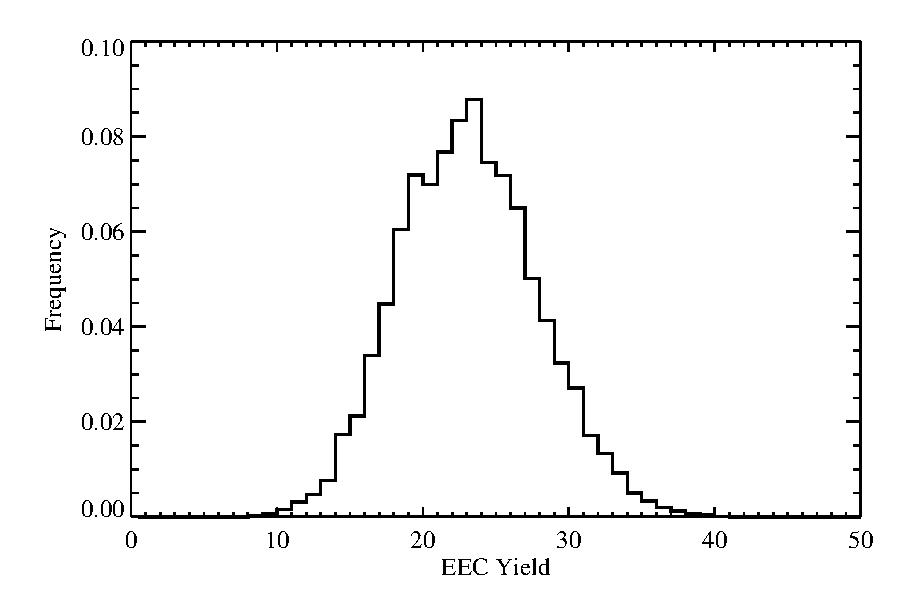
\includegraphics[width=\linewidth]{../ComparePublishedFigures/reference/starkFigure04.pdf}\end{minipage}\hfill
\begin{minipage}{0.48\textwidth}\centering\textbf{This model}\\[2pt]
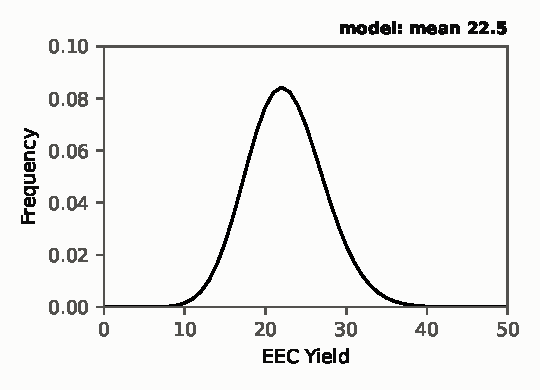
\includegraphics[width=\linewidth]{figMatchStarkFig04.pdf}\end{minipage}
\caption{Exoplanet sampling only: $A_G = 0.2$, exozodi fixed at 3 zodis, Poisson counting. Published mean 22.5, standard deviation 21\% of the mean. Model mean 22.5, which is \emph{tuned}: $\kappa$ is fitted to 22.5.}
\label{fig:pair04}
\end{figure}

\begin{figure}[htbp]
\centering
\begin{minipage}{0.48\textwidth}\centering\textbf{Stark et al.\ (2024) Fig.~7}\\[2pt]
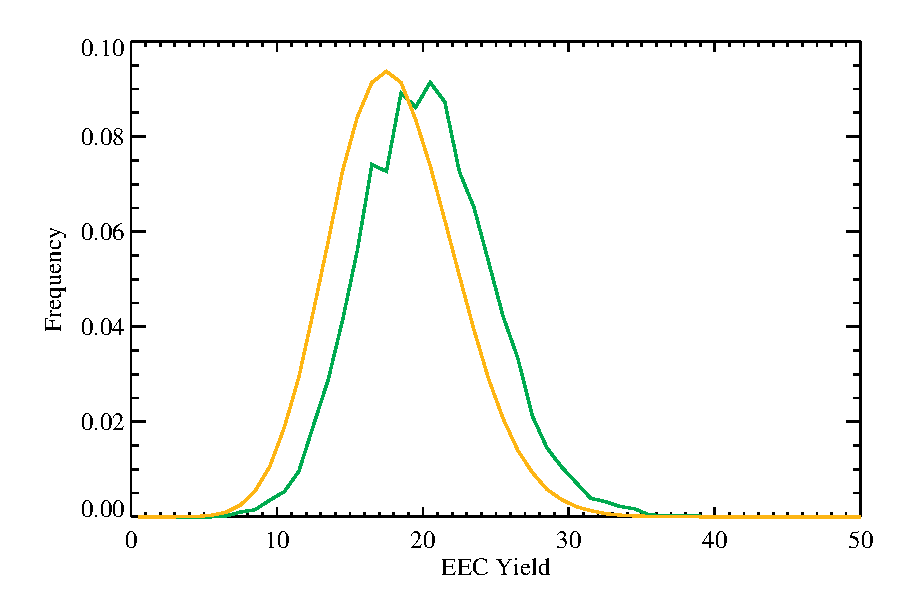
\includegraphics[width=\linewidth]{../ComparePublishedFigures/reference/starkFigure07.pdf}\end{minipage}\hfill
\begin{minipage}{0.48\textwidth}\centering\textbf{This model}\\[2pt]
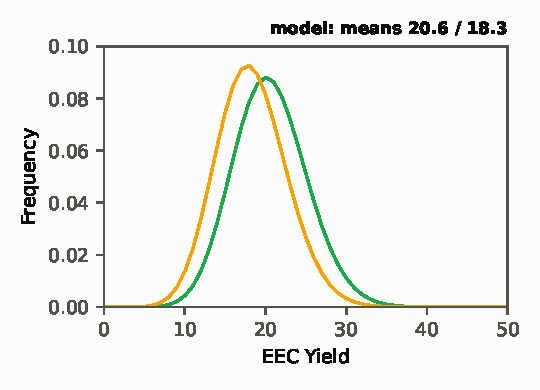
\includegraphics[width=\linewidth]{figMatchStarkFig07.pdf}\end{minipage}
\caption{Albedo drawn with exozodi fixed (green), and exozodi drawn as well (orange), $\eta_\oplus$ fixed. Published means 19.8 and 17.6. Model means 20.6 and 18.3 over 200 draws.}
\label{fig:pair07}
\end{figure}

\begin{figure}[htbp]
\centering
\begin{minipage}{0.48\textwidth}\centering\textbf{Stark et al.\ (2024) Fig.~9}\\[2pt]
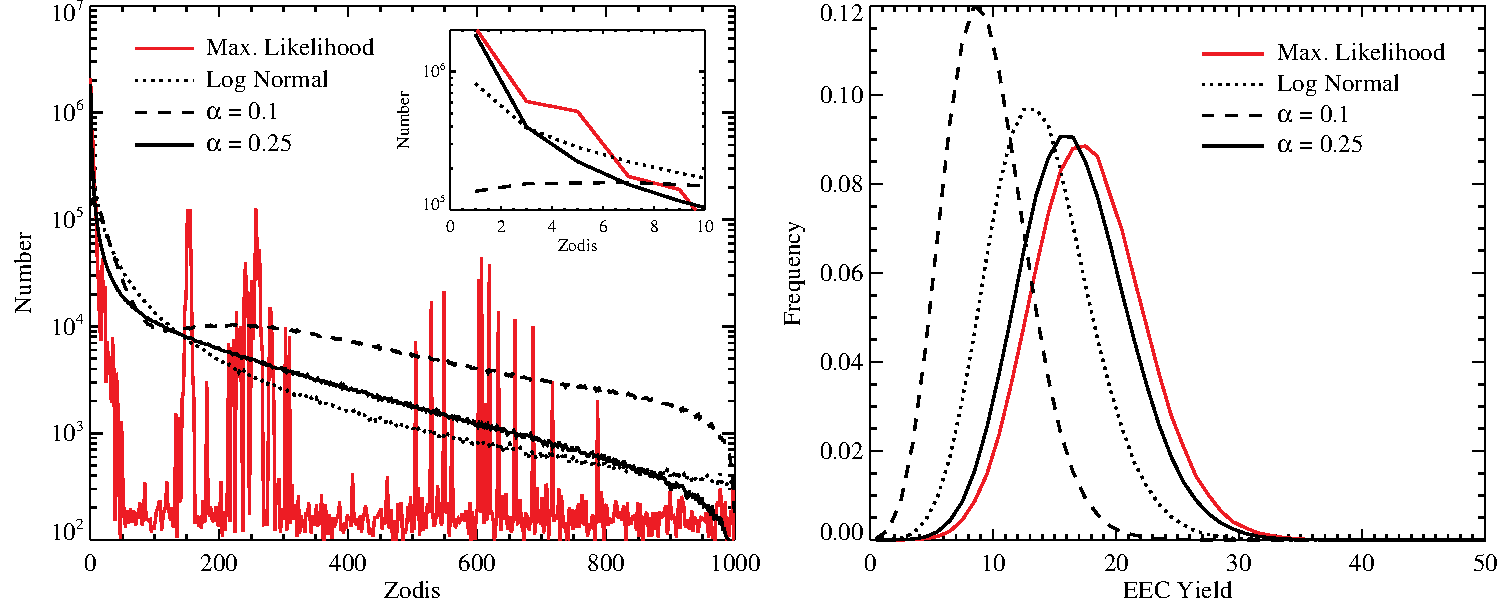
\includegraphics[width=\linewidth]{../ComparePublishedFigures/reference/starkFigure09.pdf}\end{minipage}\hfill
\begin{minipage}{0.48\textwidth}\centering\textbf{This model}\\[2pt]
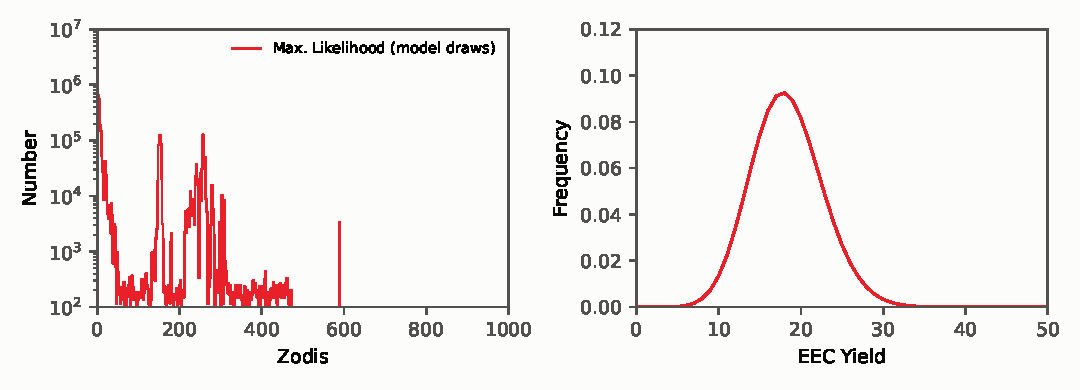
\includegraphics[width=\linewidth]{figMatchStarkFig09.pdf}\end{minipage}
\caption{Left: exozodi levels drawn from the LBTI HOSTS maximum-likelihood distribution (red); the model panel is the histogram of the levels the pipeline actually drew, scaled to Stark's $500\times10^4$ draws (median 3.00 zodis; Stark's other three distributions are not modelled). Right: the $\eta_\oplus$-fixed yield those levels produce (red).}
\label{fig:pair09}
\end{figure}

\begin{figure}[htbp]
\centering
\begin{minipage}{0.48\textwidth}\centering\textbf{Stark et al.\ (2024) Fig.~10}\\[2pt]
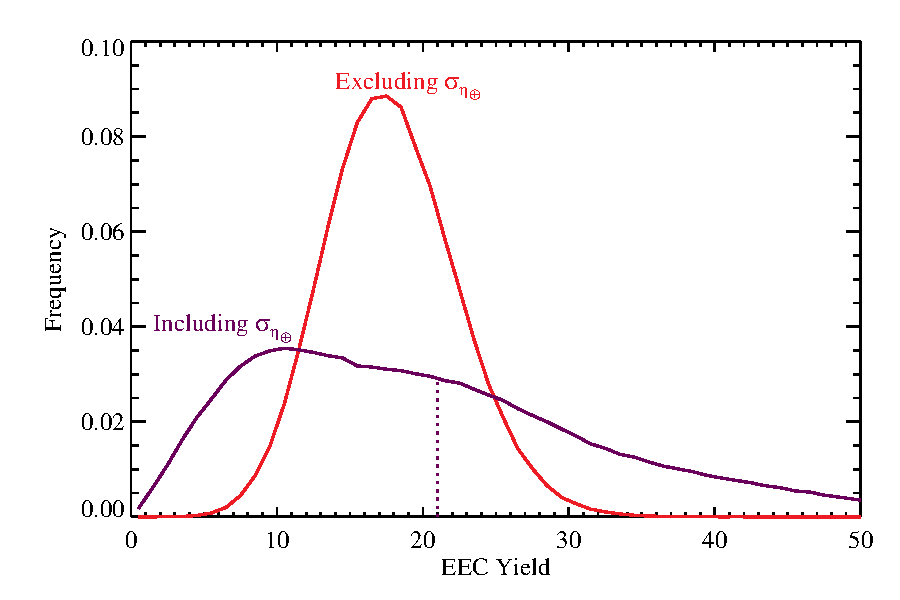
\includegraphics[width=\linewidth]{../ComparePublishedFigures/reference/starkFigure10.pdf}\end{minipage}\hfill
\begin{minipage}{0.48\textwidth}\centering\textbf{This model}\\[2pt]
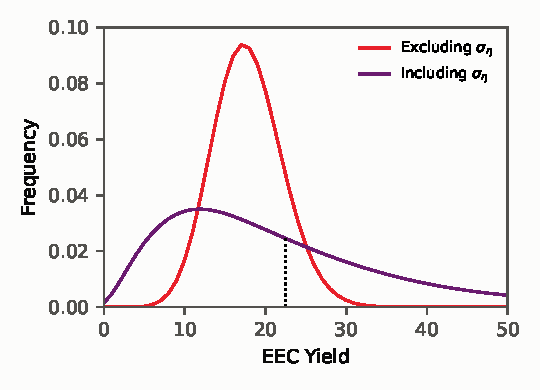
\includegraphics[width=\linewidth]{figMatchStarkFig10.pdf}\end{minipage}
\caption{Realized yield including (purple) and excluding (red) $\eta_\oplus$ uncertainty; the dotted line marks the purple mean. Total-variation distance, model to published: 0.034 (purple), 0.097 (red). Means: published 21.0 / 17.3, model 22.5 / 18.4.}
\label{fig:pair10}
\end{figure}

\begin{figure}[htbp]
\centering
\begin{minipage}{0.48\textwidth}\centering\textbf{Stark et al.\ (2024) Fig.~11}\\[2pt]
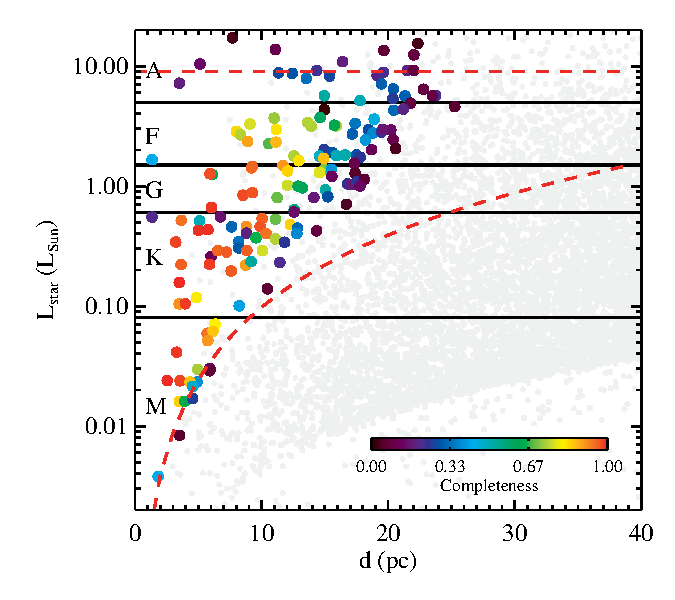
\includegraphics[width=\linewidth]{../ComparePublishedFigures/reference/starkFigure11.pdf}\end{minipage}\hfill
\begin{minipage}{0.48\textwidth}\centering\textbf{This model}\\[2pt]
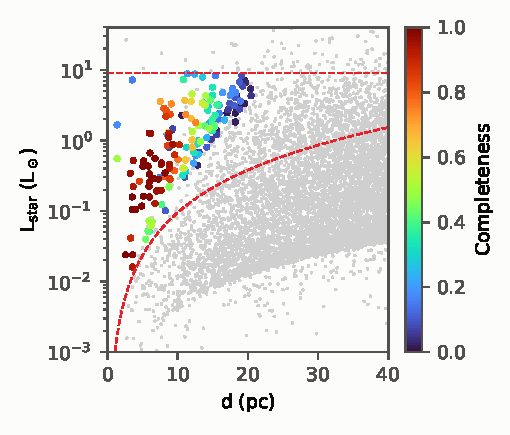
\includegraphics[width=\linewidth]{figMatchStarkFig11.pdf}\end{minipage}
\caption{Targets selected in one representative exozodi draw, coloured by completeness, over the input list in grey. Published: 154 targets, summed completeness 77.4, median 0.50. Model (draw 99, the median-yield draw): 157 targets, summed 83.5, median 0.24 over the 141 matched targets. Red dashed lines: the noise floor for a 1.4\,$R_\oplus$ planet at the EEID, and the HZ outer edge at 1.5\,$\lambda/D$ at 1\,$\mu$m; the spectral-type lines are not redrawn.}
\label{fig:pair11}
\end{figure}

\begin{figure}[htbp]
\centering
\begin{minipage}{0.48\textwidth}\centering\textbf{Stark et al.\ (2024) Fig.~12}\\[2pt]
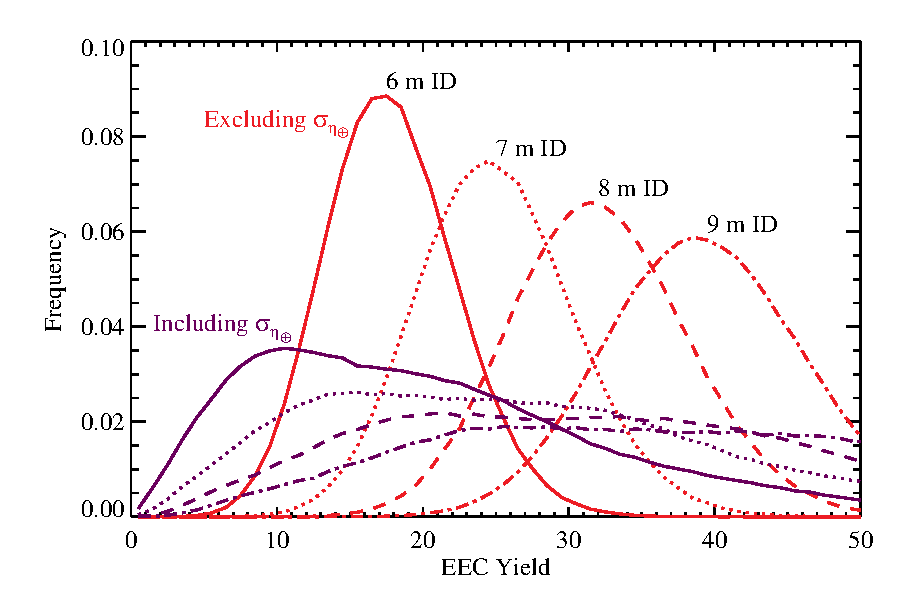
\includegraphics[width=\linewidth]{../ComparePublishedFigures/reference/starkFigure12.pdf}\end{minipage}\hfill
\begin{minipage}{0.48\textwidth}\centering\textbf{This model}\\[2pt]
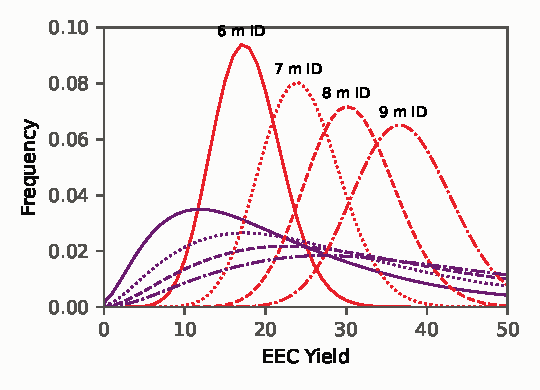
\includegraphics[width=\linewidth]{figMatchStarkFig12.pdf}\end{minipage}
\caption{Realized yield at 6, 7, 8 and 9\,m inscribed diameter (solid, dotted, dashed, dot-dashed), including (purple) and excluding (red) $\sigma_{\eta_\oplus}$, with the calibration frozen at 6\,m. Published: excluding $\sigma_{\eta_\oplus}$, 9\,m gives 2.2 times the 6\,m yield; model 2.04 times.}
\label{fig:pair12}
\end{figure}

\begin{figure}[htbp]
\centering
\begin{minipage}{0.48\textwidth}\centering\textbf{Stark et al.\ (2024) Fig.~14}\\[2pt]
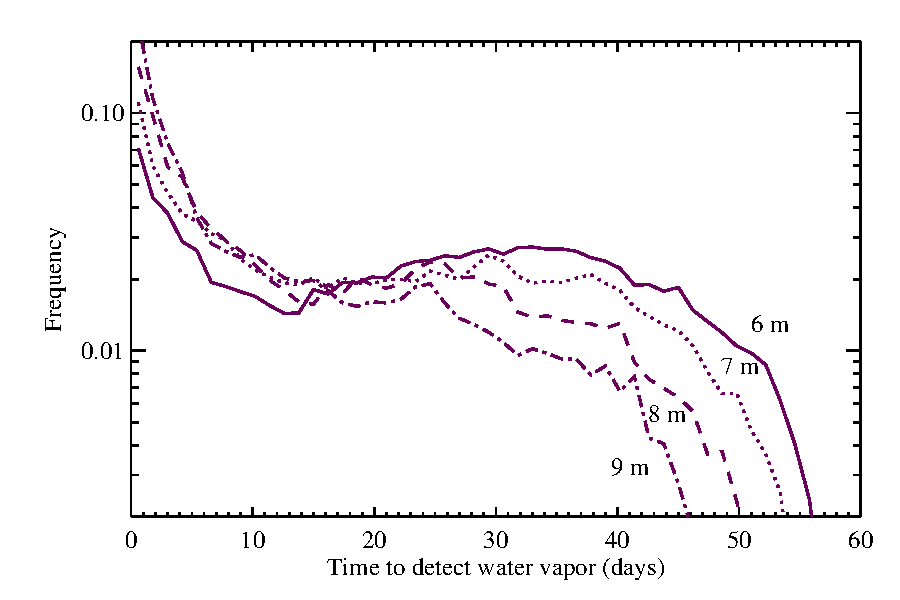
\includegraphics[width=\linewidth]{../ComparePublishedFigures/reference/starkFigure14.pdf}\end{minipage}\hfill
\begin{minipage}{0.48\textwidth}\centering\textbf{This model}\\[2pt]
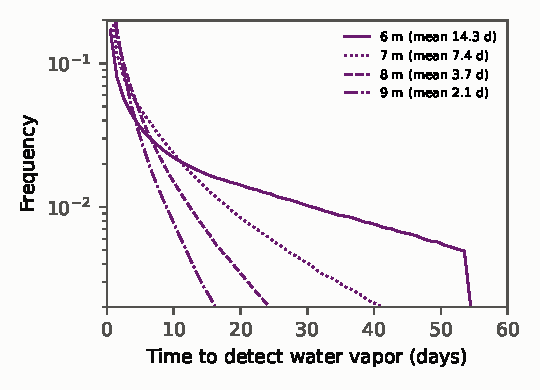
\includegraphics[width=\linewidth]{figMatchStarkFig14.pdf}\end{minipage}
\caption{Characterization times of individual EECs among the first 18 at 6--9\,m (model: 20 exozodi draws re-derived planet by planet, 1-day bins). Published means 22 and 3.5 days at 6 and 9\,m; model means at 6/7/8/9\,m: 13.8 / 6.7 / 3.3 / 1.8 days. Stark does not state his normalization, and with 1-day bins his 9\,m plateau alone would exceed his stated mean, so compare shapes, not heights: his distributions keep a plateau of 15--50-day spectra at every aperture, which the model's lack.}
\label{fig:pair14}
\end{figure}

\begin{figure}[htbp]
\centering
\begin{minipage}{0.48\textwidth}\centering\textbf{Stark et al.\ (2024) Fig.~15}\\[2pt]
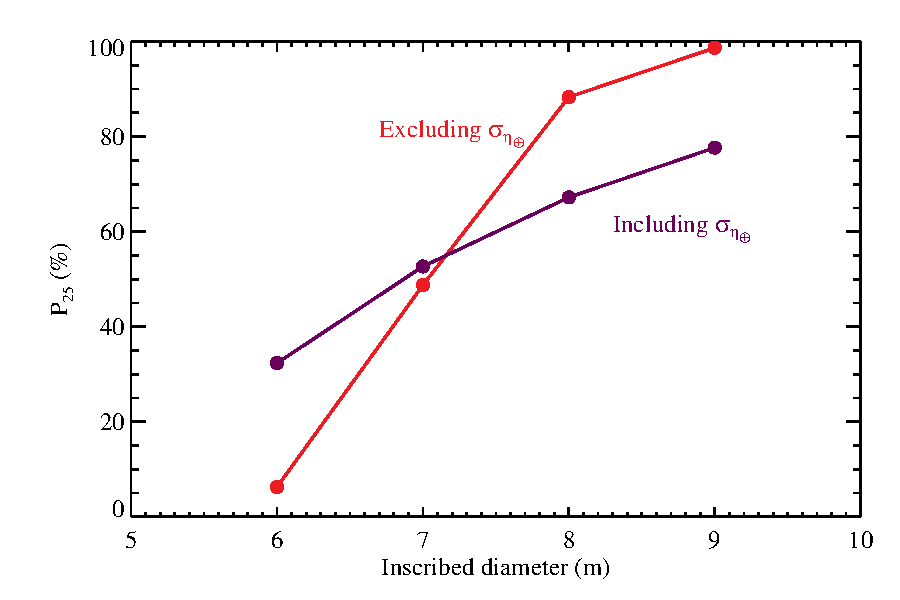
\includegraphics[width=\linewidth]{../ComparePublishedFigures/reference/starkFigure15.pdf}\end{minipage}\hfill
\begin{minipage}{0.48\textwidth}\centering\textbf{This model}\\[2pt]
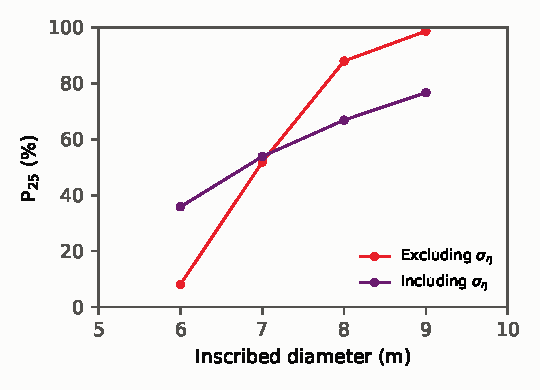
\includegraphics[width=\linewidth]{figMatchStarkFig15.pdf}\end{minipage}
\caption{$P_{25}$ against inscribed diameter. Published including $\sigma_{\eta_\oplus}$ 32/53/67/78\%, model 36 / 54 / 67 / 77\%; excluding, published 6/49/89/99.5\%, model 8 / 52 / 88 / 99\%.}
\label{fig:pair15}
\end{figure}

\begin{figure}[htbp]
\centering
\begin{minipage}{0.48\textwidth}\centering\textbf{Stark et al.\ (2024) Fig.~25}\\[2pt]
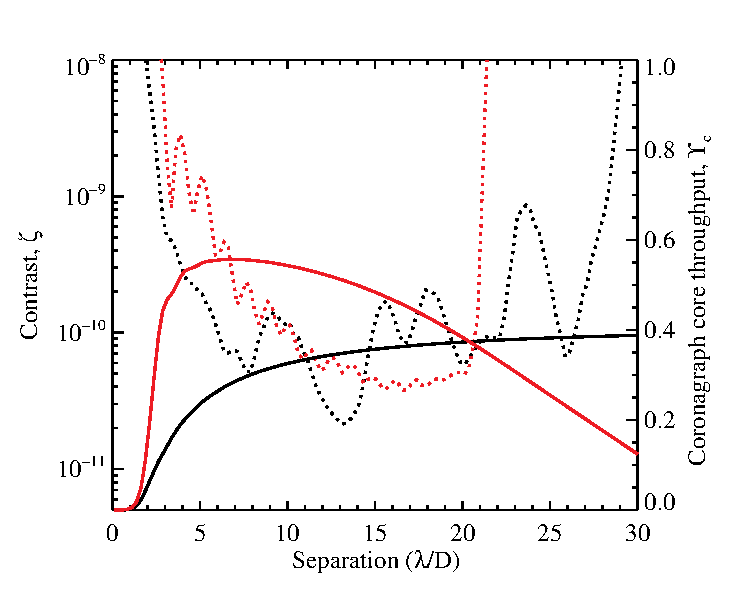
\includegraphics[width=\linewidth]{../ComparePublishedFigures/reference/starkFigure25.pdf}\end{minipage}\hfill
\begin{minipage}{0.48\textwidth}\centering\textbf{This model}\\[2pt]
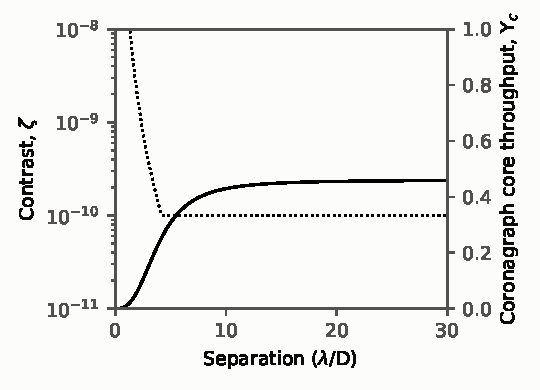
\includegraphics[width=\linewidth]{figMatchStarkFig25.pdf}\end{minipage}
\caption{DMVC6 raw contrast (dotted) and core throughput (solid) against separation in circumscribed $\lambda/D$. The model curves are the digitized published ones, so this pair checks the digitization, not the model. The model's contrast is shown with the $10^{-10}$ floor applied, as the exposure times use it; the published curve is the raw simulation. The published figure also shows the PIAA-FPM2.5 (red), which is not used.}
\label{fig:pair25}
\end{figure}

%======================================================================
\section{Results}
\label{sec:results}

\begin{figure}[htbp]
\centering
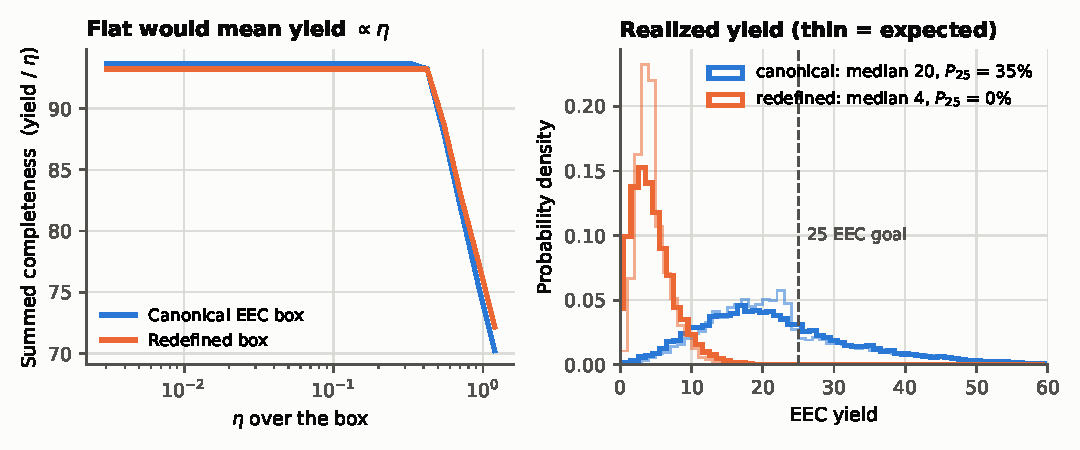
\includegraphics[width=\textwidth]{figYieldPrediction.pdf}
\caption{Left: summed completeness against $\eta$; its decline is the characterization burden
consuming search time, i.e.\ the $\eta_\oplus \to \lambda$ edge of Fig.~\ref{fig:pgm}. Right: the
realized yield distributions, Eq.~\eqref{eq:thinning} marginalized over $\eta_\oplus$ (heavy), and
the expected yield $\Lambda$ alone (thin).}
\label{fig:yieldprediction}
\end{figure}

\begin{figure}[htbp]
\centering
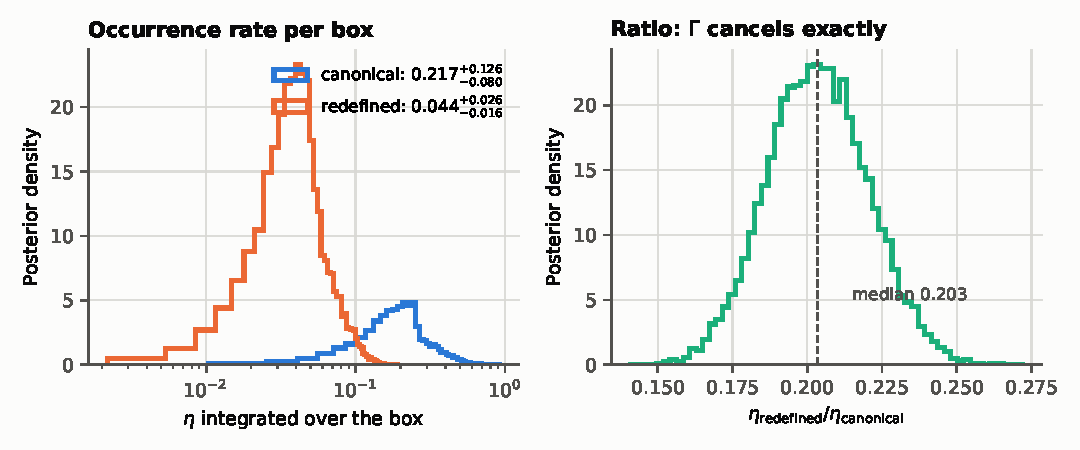
\includegraphics[width=\textwidth]{figOccurrencePosterior.pdf}
\caption{Left: the occurrence rate integrated over each box. Right: their ratio $\rho_\mathcal{B}$,
tight because $\Gamma$ cancels.}
\end{figure}

\subsection{Why the yield ratio exceeds the occurrence ratio}
\label{sec:ratio}

The occurrence ratio $0.204$ decomposes into about 0.32 from narrowing the habitable zone
and 0.63 from the mass selection. The yield ratio, $0.245$, is larger, for three reasons that
are all visible in Fig.~\ref{fig:pgm}:
\begin{enumerate}
\item \textbf{Freed characterization time} ($\eta_\mathcal{B} \to \lambda$). Fewer expected
detections leave more of the budget for searching. Raises the ratio.
\item \textbf{The faintest planets are removed} ($\mathcal{B} \to \mathbf{o}_{ij}$). Truncating at
1.20 scaled AU removes planets up to $(1.67/1.20)^2 \approx 1.9$ times fainter than those
kept. Raises the ratio.
\item \textbf{Distant stars are lost} ($\mathcal{B} \to C_i$). For distant stars only the outer
habitable zone clears the inner working angle. Lowers the ratio.
\end{enumerate}
The first two win. Under the redefined selection a 6\,m telescope reaches 25 candidates with
probability 1.19\%: a narrow habitable zone and a mass-selected sample put the decadal
benchmark out of reach at this aperture for any plausible $\eta_\oplus$.

%======================================================================
\section{The Earth zone and the classic habitable zone, star by star}
\label{sec:earthzone}

The \emph{Earth zone} is this report's redefined box: 0.96--1.20~AU for the Sun, scaled by
$\sqrt{L_\star}$, holding planets of 0.5--2\,$M_\oplus$. The \emph{classic habitable zone} is
Stark's canonical box, 0.95--1.67~AU scaled the same way, holding planets up to 1.4\,$R_\oplus$.
Step A11 tabulates both for every one of the 1,500 screened stars, in AU, in
milliarcseconds and in $\lambda/D$ of the 6\,m telescope at 550 and 1000\,nm, together with what
each zone's own optimized survey expects to find there: each box's survey is re-optimized in every
exozodi draw at its posterior-median occurrence rate ($\eta = 0.255$ and 0.0520), and a
star's expected yield is $\eta$ times its completeness averaged over draws. The full table is
\texttt{TabulateEarthZones/earthZoneTable.csv}; Appendix~\ref{app:stars} lists the
183 stars that contribute in either survey.

\textbf{Totals.} The Earth zone is a third as wide as the classic zone in scaled AU and holds
0.204 as many candidates per star. Summed over stars the expected yield is
19.30 in the classic zone and 4.63 in the Earth zone, a ratio of 0.240;
star by star the ratio has median 0.241 (68\% of stars between 0.201 and
0.325). The classic survey observes 184 stars in at least half the draws at a
mean completeness of 0.45; the Earth-zone survey observes 171 at 0.54. The
narrower zone is easier to complete, because its planets sit closer in and are brighter, so the
survey concentrates on slightly fewer stars and reaches a larger fraction of their candidates. The
ratio rises from about 0.21 for the faintest, nearest stars to about 0.33 for stars above
$5\,L_\odot$ (Table~\ref{tab:earthzone}): around distant and luminous stars the classic zone's
outer planets are too faint to be found, so losing them costs little.

\textbf{Angle.} The Earth zone sits at the inner edge of the classic zone, so in angle it is the
harder part of it. With the half-throughput inner working angle at 2.93\,$\lambda/D$
(inscribed), a mean 91\% of the Earth zone lies outside it at 550\,nm against
96\% of the classic zone, and at 1000\,nm, where water is sought,
47\% against 64\%, averaged over the stars either survey observes. The
coronagraph still passes light inside that angle, which is why the loss in yield is smaller than
the loss in angle.

\begin{table}[htbp]
\centering
\small
\begin{tabular}{lrrrrrr}
\toprule
& & \multicolumn{2}{c}{\textbf{stars observed}} & \multicolumn{2}{c}{\textbf{expected EECs}} & \\
\textbf{Luminosity ($L_\odot$)} & \textbf{stars} & \textbf{classic} & \textbf{Earth} & \textbf{classic} & \textbf{Earth} & \textbf{ratio} \\
\midrule
L $<$ 0.3 & 47 & 36 & 33 & 5.57 & 1.15 & 0.21 \\
0.3-0.6 & 75 & 30 & 26 & 4.11 & 0.91 & 0.22 \\
0.6-1 & 102 & 19 & 17 & 1.95 & 0.44 & 0.23 \\
1-2 & 294 & 33 & 30 & 3.13 & 0.78 & 0.25 \\
2-5 & 665 & 44 & 42 & 3.72 & 1.07 & 0.29 \\
L $>$ 5 & 317 & 22 & 23 & 0.82 & 0.27 & 0.33 \\
\midrule
\textbf{Distance} & & & & & & \\
\midrule
$<$ 5 pc & 15 & 15 & 15 & 2.97 & 0.66 & 0.22 \\
5-10 pc & 59 & 59 & 57 & 9.60 & 2.16 & 0.23 \\
10-15 pc & 95 & 65 & 58 & 5.16 & 1.37 & 0.27 \\
15-20 pc & 133 & 42 & 37 & 1.50 & 0.42 & 0.28 \\
$>$ 20 pc & 1198 & 3 & 4 & 0.08 & 0.02 & 0.21 \\
\bottomrule
\end{tabular}
\caption{Where each zone's yield comes from. ``Observed'' means allocated time in at least half of
the exozodi draws. Each zone's survey is optimized for its own candidates.}
\label{tab:earthzone}
\end{table}

\begin{figure}[htbp]
\centering
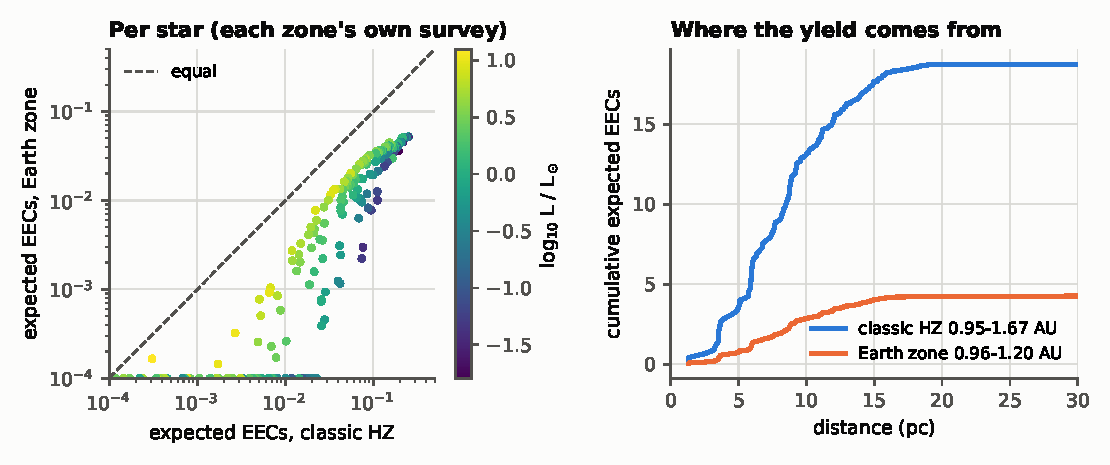
\includegraphics[width=\textwidth]{figEarthZones.pdf}
\caption{Left: each star's expected Earth-zone yield against its classic-zone yield, coloured by
luminosity. Right: cumulative expected yield with distance for both zones.}
\label{fig:earthzone}
\end{figure}

%======================================================================
\section{The open problem: characterization time and the target mix}
\label{sec:open}

With $\kappa$ explained and exozodi marginalized, the level problem of earlier revisions is gone:
the fixed-$\eta_\oplus$ yield is 18.30 against Stark's 17.35 (5.5\% high,
inside the 10\% the researcher set as the target), the exozodi penalty is 11.2\% against
11.1\%, and $P_{25}$ agrees at every aperture. What remains is one discrepancy seen three ways.

\textbf{The symptom.} The mean characterization time of the first 18 EECs is 13.8\,d at
6\,m and 1.85\,d at 9\,m, against Stark's 22 and 3.5 (Sec.~4.1): the easiest targets are
characterized too fast, by a factor of about two. The shape says where the difference is
(Fig.~\ref{fig:pair14}): Stark's first 18 EECs include a plateau of 15--50-day spectra at every
aperture, while this model's individual characterization times fall away steeply, with almost
none above about 15 days at 9\,m. The peak of the realized
distribution sits at 14 rather than 10.

\textbf{The target mix differs.} Against Stark's Fig.~11 (Fig.~\ref{fig:pair11}), in the same
characterization-gated completeness and one representative exozodi draw, this model matches the
nearest stars --- median 0.98 against 0.95 inside 6\,pc --- but gives stars at
10--15\,pc a median of 0.35 (published 0.73) and at 15--20\,pc 0.07
(0.28). By luminosity, stars of $1$--$2\,L_\odot$ get 0.08 (published 0.62)
and stars of $2$--$5\,L_\odot$ get 0.14 (0.47), with 42\% of the latter
allocated essentially nothing. The survey concentrates on nearby stars instead, and reaches
Stark's total by completing them more fully.

\textbf{The cause is characterization cost.} At $R = 140$ near 1\,$\mu$m the characterization
background is exozodi-dominated, and the exozodi count rate is a surface brightness, nearly the
same for every star, while the planet dims as $d^{-2}$; characterization time therefore grows
roughly as $d^4$. For an Earth twin at quadrature the exozodi-to-planet count ratio per spectral
bin is 1.3 at $\tau$~Cet, 7 at 61~Vir, 20 at $\theta$~Boo and
36 at 110~Her, and the characterization times are 0.21, 10,
72 and 255 days against a 60-day cap. Distant, luminous targets are priced
out of the survey while nearby ones are characterized in hours to days.

\textbf{Ruled out, each by direct test.}
\begin{itemize}
\item \emph{The noise floor}: removing it entirely leaves luminous-star completeness unchanged.
\item \emph{The detector saturation definition}: Stark (2019) sets $\mathrm{CR_{sat}}$ to ten times
an Earth twin's core-pixel rate, where this model uses the scene; characterization times change by
under 1\%.
\item \emph{IFS pixels}: 96 per spectral bin matches Stark (2024) Table~2. Latouf et al.\ (2026)
use 6 for a different instrument.
\item \emph{Detector noise generally}: Stark's Scenario~D (Skipper CCD) gains 1.5$\times$ in
characterization time, which his text attributes mostly to a 30\% throughput gain; the implied
detector share, about 12\%, matches this model's.
\item \emph{The first-18 ordering}: ordering targets by survey priority rather than by
characterization cost changes the mean by 1\%.
\item \emph{The Fig.~11 metric}: detection-only completeness fixes the low-luminosity stars but not
the luminous ones.
\item \emph{Dust colour}: the zero point is a solar-coloured source normalized at $V$, which is the
treatment Stark (2015) describes.
\end{itemize}

\textbf{Not the calibration.} Before this revision $\kappa = 1.62$ multiplied spectra as well as
detections, and the obvious suspicion was that it sped up the easy spectra. It did, but removing it
through the $T_{\rm sky}$ map left the first-18 times unchanged (Sec.~\ref{sec:calibration}), and no
single factor on spectra can change their 6\,m/9\,m ratio, 7.5 here against 6.2.

\textbf{Reading.} The model's characterization time rises with target difficulty more steeply than
Stark's: nearby targets are cheaper and distant ones dearer. Both ends move the same way under the
exozodi-limited $d^4$ scaling above, which this model follows closely; Stark's numbers behave as if
something flattens that dependence. Detector noise, the obvious candidate, is argued against in
the list above; what remains untested includes how Stark schedules a spectrum against the planet's
orbit (this model takes the most favourable of 40 phases, which is the cheapest possible choice),
whether his S/N per spectral bin counts one bin or a band average, and the exozodi surface
brightness at the planet's own separation: Stark (2019) Table~1 notes that it ``varies with
spectral type and planet-star separation'', while this model evaluates it at the EEID. Those are
the next things to test. By
the standard this project has held to, a fix must move the first-18 times at both apertures, the
distant targets of Fig.~11 and the peak of Fig.~10 together.

%======================================================================
\section{Limitations}

\begin{itemize}
\item \textbf{$T_{\rm sky}(r)$ is reconstructed.} Stark's map comes from 2-D PSF simulations that
are not published; this model scales the azimuthally averaged core-throughput curve, which assumes
a separation-independent core fraction and omits the convolution's smoothing. It removed the need
for $\kappa$ (now 0.988), but a different reconstruction would move the absolute yields.
\item \textbf{The coronagraph is azimuthally averaged.} The digitized one-dimensional DMVC6 curves
stand in for two-dimensional maps.
\item \textbf{Exozodi draws are interpolated.} 200 draws (Stark: 500) evaluated on a
23-level grid; interpolation changes optimized yields by at most 0.24\%. Stark also draws
the HOSTS distribution itself from its posterior, which he finds negligible and which is not
modelled.
\item \textbf{The $\eta_\oplus$ distribution is reconstructed.} Its width is inferred from Stark's
Fig.~10 because the Bryson chains are unpublished; the text's 86\% reading is one option away.
\item \textbf{$\alpha, \beta$ are prior-dominated.} The ratio $\rho_\mathcal{B}$ inherits SAG13's
shape, not a re-fit to Kepler DR25.
\item \textbf{The area fill factor (0.785) is unsourced.} It moves the yield by about $\pm$4\%.
\end{itemize}

%======================================================================
\section{Reproducing this}

The project is a twelve-step vaibify pipeline in \texttt{/workspace/yields}. Every step declares its
inputs and outputs and carries integrity, qualitative and quantitative tests generated from its
outputs; the physics library carries 78 unit tests. Every number in this report is injected from
a step or exploration output at build time (\texttt{cd doc \&\& python3 buildReport.py}), so a
re-run cannot leave a stale claim in print.

\begin{table}[htbp]
\centering
\small
\begin{tabular}{llp{8.6cm}}
\toprule
\textbf{Step} & \textbf{Name} & \textbf{Nodes of Fig.~\ref{fig:pgm} it implements} \\
\midrule
A01 & buildTargetCatalog & $\mathbf{s}_i$: HPIC, 11,757 stars \\
A02 & modelCoronagraph & $\mathcal{M}$, $\mathcal{B}$, $p_z$ (digitized Fig.~9), pinned $z_i$, $p_A$ \\
A03 & calibrateToStark & $\kappa$, at fixed exozodi \\
A04 & computeCompleteness & $\mathbf{o}_{ij}$, $A_{ij}$, $\boldsymbol{\tau}_{ij}$, $C_i$ on a grid of $z$; 200 draws of $\mathbf{z}$ \\
A05 & optimizeSurvey & $\lambda$, $\mathbf{a}_i$ at $\eta = 0.24$, at fixed $z$ and per draw \\
A06 & sampleOccurrencePosterior & $\eta_\oplus$, $\alpha,\beta$, $\rho_\mathcal{B}$ \\
A07 & predictRedefinedYield & $\mathbf{a}_i(\eta)$ on a grid, $Y$ by Eq.~\eqref{eq:thinning} \\
A08 & compareApertureScaling & the same at 6--9\,m with $\kappa$ frozen, over draws of $\mathbf{z}$ \\
A09 & verifyAgainstPublished & Table~\ref{tab:verif} \\
A10 & compareTargetCompleteness & per-target comparison with Fig.~11 \\
A11 & tabulateEarthZones & Sec.~\ref{sec:earthzone}, Appendix~\ref{app:stars} \\
A12 & comparePublishedFigures & Sec.~\ref{sec:pairs} \\
\bottomrule
\end{tabular}
\caption{Pipeline steps mapped onto the graphical model.}
\end{table}

%======================================================================
\appendix
\section{Ledger of hypotheses}
\label{app:ledger}

Every proposed explanation for a disagreement with the published record, with its outcome. A
defect can be genuine, worth fixing, and irrelevant to the symptom that led to it, so ``real error,
not the cause'' is kept separate from ``the cause''.

\begin{table}[htbp]
\centering
\scriptsize
\begin{tabular}{p{4.6cm}p{2.6cm}p{8.0cm}}
\toprule
\textbf{Hypothesis} & \textbf{Outcome} & \textbf{Evidence} \\
\midrule
Missing revisits & \textbf{Real, a cause} & Single-visit only; modelling up to six visits raised the uncalibrated yield 1.7$\times$. \\
Characterization-time statistic & \textbf{Real, a cause} & A median over all detectable planets, where the budget needs a mean over those counted; $D^{1.11} \to D^{1.88}$. \\
Over-cap characterization charged & \textbf{Real, a cause} & 15\,000 days charged at 20\,pc for an observation never attempted. \\
Reconstructed target catalog & \textbf{Real, a cause} & HPIC was reachable; the Gaia stand-in lacked 26--34\% of distant FGK dwarfs and ran hot. \\
Coronagraph aperture convention & \textbf{Real, the cause} & Curves are in circumscribed $\lambda/D$; the IWA sat 19\% too far out. Yield 14.7 $\to$ 18.7. \\
Collecting area as inscribed circle & \textbf{Real, partial} & Charged the Lyot discard twice. \\
Characterization at detection phase & \textbf{Real, a cause} & Stark (2019) Sec.~5: the orbit is known, so ``the phase of the planet could be optimized. \\
Characterization budget under albedo draw & \textbf{Real, a cause} & Stark (2024) Sec.~3.2 fixes it at $A_G = 0.2$; albedo penalty 0.050 $\to$ 0.087. \\
Constant $T_{\rm sky}$ & \textbf{Real, the cause of $\kappa$} & Stark (2019) Eqs.~5--6 make it a map; with it the uncalibrated yield is 22.61 and $\kappa$ falls 1.62 $\to$ 0.988. Characterization times barely move. \\
One exozodi draw & \textbf{Real, fixed} & Now 200 draws with the survey re-optimized per draw; exozodi penalty 11.2\% (Stark 11.1\%). \\
Split $\kappa$ (detection vs spectra) & Rejected & A scalar on spectra cannot change the 6/9\,m characterization-time ratio. \\
Exozodi drawn during calibration & \textbf{Real, a cause} & $\kappa$ fitted to a drawn-exozodi yield cancels the exozodi penalty. \\
Lognormal exozodi stand-in & \textbf{Real, a cause} & 0.2\% of stars above 100 zodis vs 21\% in HOSTS; penalty 0.7\% $\to$ 11.2\%. \\
Pinned LBTI stars omitted & \textbf{Real, partial} & Worth at most 0.47 EEC here. \\
$\eta_\oplus$ interval read as 86\% & \textbf{Real, the cause of the shape} & Fig.~10 requires $\ln$-width $\sim$0.8; distance 0.142 $\to$ 0.024. \\
Published mode ill-determined & \textbf{Rejected} & Stark's 498 runs carry 1000 planet draws each; an earlier bootstrap resampled only 498 yields. \\
Fig.~4 mean compared with the wrong yield & \textbf{Real, not the cause} & Fig.~4 is sampling only at $A_G = 0.2$; the check is now marked tuned. \\
$T_{\rm sky}$ missing; exozodi law & \textbf{Real, not the cause} & Backgrounds 1.48$\times$ too bright; constant-surface-brightness law. Together 1\%. \\
Contrast floor inside the knee & \textbf{Real, not the cause} & Floor applied universally. \\
Noise-floor screen & \textbf{Real, not the cause} & Admitted nothing above 4.6\,$L_\odot$. \\
Screening cap, uniform bias, bandpass choice & Rejected & 1.3\%, destroys 7--9\,m, 0.01. \\
Two detections for orbits & Rejected & Shifts the curve, does not narrow it. \\
Equal-slope allocation & Rejected & 0.00\% from an exact optimum. \\
Blackbody stellar flux & Rejected & +0.019\,mag against measured $V$. \\
Stark's per-visit albedo test & Rejected & Gives a weaker penalty (3.3\%). \\
Noise floor, CIC definition, IFS pixels, ordering, dust colour & Rejected & Sec.~\ref{sec:open}. \\
\bottomrule
\end{tabular}
\caption{The ledger. The traps that recur --- compensating errors, comparing against the wrong
published curve, biased diagnostic sub-samples, and read-off values --- are documented in
\texttt{doc/handoffToNextAgent.md}.}
\end{table}

\clearpage
\section{Every contributing star}
\label{app:stars}

Stars with an expected yield of at least 0.01 EEC in either zone's survey, in order of
their classic-zone yield. Zone edges are angular separations in milliarcseconds; $C$ is the
completeness reached, averaged over exozodi draws; $N$ is the expected number of candidates. The
complete table, with every screened star and every column (AU, $\lambda/D$ at 550 and 1000\,nm,
time allocated, characterization time, fraction of draws observed), is
\texttt{TabulateEarthZones/earthZoneTable.csv}.

{\scriptsize
\setlength{\tabcolsep}{3pt}
\begin{longtable}{llrrrrrrrrr}
\toprule
\textbf{Star} & \textbf{SpT} & \textbf{$d$ (pc)} & \textbf{$L$ ($L_\odot$)} & \textbf{Earth zone (mas)} & \textbf{classic HZ (mas)} & \textbf{$C_{\rm HZ}$} & \textbf{$C_{\rm EZ}$} & \textbf{$N_{\rm HZ}$} & \textbf{$N_{\rm EZ}$} & \textbf{ratio} \\
\midrule
\endhead
tau Cet & G8V & 3.65 & 0.52 & 189--237 & 188--330 & 0.98 & 1.00 & 0.247 & 0.052 & 0.21 \\
HD  95735 & M2+V & 2.55 & 0.0239 & 58--73 & 58--101 & 0.98 & 1.00 & 0.245 & 0.052 & 0.21 \\
eps Ind & K5V & 3.64 & 0.222 & 124--155 & 123--216 & 0.98 & 1.00 & 0.245 & 0.052 & 0.21 \\
61 Cyg A & K5V & 3.50 & 0.158 & 109--136 & 108--190 & 0.97 & 1.00 & 0.244 & 0.052 & 0.21 \\
61 Cyg B & K7V & 3.50 & 0.104 & 89--111 & 88--154 & 0.97 & 1.00 & 0.242 & 0.052 & 0.21 \\
HD 217987 & M2V & 3.29 & 0.0413 & 59--74 & 59--103 & 0.96 & 1.00 & 0.239 & 0.052 & 0.22 \\
70 Oph A & K0V & 5.11 & 0.514 & 135--168 & 133--234 & 0.95 & 1.00 & 0.235 & 0.051 & 0.22 \\
del Equ & F7(V)+G & 4.51 & 0.265 & 110--137 & 108--191 & 0.95 & 1.00 & 0.233 & 0.051 & 0.22 \\
V* AX Mic & M1V & 3.97 & 0.105 & 78--98 & 77--136 & 0.94 & 1.00 & 0.232 & 0.051 & 0.22 \\
omi02 Eri & K0V & 5.01 & 0.428 & 125--157 & 124--218 & 0.95 & 1.00 & 0.232 & 0.051 & 0.22 \\
eps Eri & K2V & 3.22 & 0.342 & 174--218 & 173--303 & 0.94 & 1.00 & 0.229 & 0.051 & 0.22 \\
70 Oph B & K4V & 5.10 & 0.162 & 76--95 & 75--132 & 0.91 & 0.99 & 0.223 & 0.051 & 0.23 \\
e Eri & G6V & 6.04 & 0.663 & 129--162 & 128--225 & 0.91 & 0.99 & 0.221 & 0.051 & 0.23 \\
eta Cas & F9V & 5.92 & 1.27 & 182--228 & 181--317 & 0.90 & 0.99 & 0.218 & 0.051 & 0.23 \\
36 Oph & K2V+K1V & 5.95 & 0.334 & 93--117 & 92--162 & 0.89 & 0.97 & 0.218 & 0.050 & 0.23 \\
sig Dra & K0V & 5.76 & 0.433 & 110--137 & 108--191 & 0.89 & 0.99 & 0.217 & 0.051 & 0.23 \\
del Pav & G8IV & 6.10 & 1.25 & 176--220 & 174--306 & 0.89 & 0.99 & 0.216 & 0.051 & 0.23 \\
IRAS 20079-3614 &  & 6.01 & 0.26 & 81--102 & 81--142 & 0.88 & 0.95 & 0.215 & 0.049 & 0.23 \\
HD 131977 & K4V & 5.89 & 0.223 & 77--96 & 76--134 & 0.87 & 0.95 & 0.212 & 0.049 & 0.23 \\
HD  88230 & K6VeFe- & 4.87 & 0.117 & 68--84 & 67--118 & 0.88 & 0.98 & 0.212 & 0.050 & 0.23 \\
36 Oph B & K1V & 5.95 & 0.331 & 93--116 & 92--162 & 0.87 & 0.97 & 0.212 & 0.049 & 0.23 \\
ksi Boo & G7Ve+K5 & 6.75 & 0.554 & 106--132 & 105--184 & 0.86 & 0.93 & 0.210 & 0.048 & 0.23 \\
V* GX And & M2V & 3.56 & 0.0239 & 42--52 & 41--72 & 0.85 & 0.89 & 0.206 & 0.046 & 0.22 \\
HD 219134 & K3V & 6.54 & 0.29 & 79--99 & 78--137 & 0.84 & 0.90 & 0.205 & 0.046 & 0.22 \\
V* V2215 Oph & K5V & 5.95 & 0.158 & 64--80 & 63--111 & 0.83 & 0.89 & 0.202 & 0.045 & 0.22 \\
107 Psc & K1V & 7.64 & 0.458 & 85--106 & 84--148 & 0.82 & 0.88 & 0.200 & 0.045 & 0.23 \\
bet CVn & G0V & 8.47 & 1.22 & 125--156 & 124--218 & 0.79 & 0.86 & 0.193 & 0.044 & 0.23 \\
61 Vir & G6.5V & 8.53 & 0.841 & 103--129 & 102--179 & 0.79 & 0.84 & 0.191 & 0.043 & 0.23 \\
mu. Cas & G5Vb & 7.68 & 0.479 & 87--108 & 86--151 & 0.78 & 0.83 & 0.189 & 0.042 & 0.22 \\
HD  16160 & K3V & 7.23 & 0.282 & 71--88 & 70--123 & 0.76 & 0.80 & 0.185 & 0.041 & 0.22 \\
HD 173739 & M3V & 3.52 & 0.016 & 35--43 & 34--60 & 0.76 & 0.72 & 0.183 & 0.037 & 0.20 \\
chi01 Ori & G0V & 8.70 & 1.11 & 116--145 & 115--202 & 0.74 & 0.80 & 0.180 & 0.041 & 0.23 \\
ksi UMa A & F8.5:V & 8.73 & 1.26 & 123--154 & 122--214 & 0.74 & 0.81 & 0.179 & 0.041 & 0.23 \\
HD 156384 & K3V+K5V & 6.97 & 0.192 & 60--76 & 60--105 & 0.74 & 0.77 & 0.178 & 0.040 & 0.22 \\
chi Dra & F7V & 8.30 & 2.19 & 171--214 & 170--298 & 0.73 & 0.85 & 0.175 & 0.043 & 0.25 \\
ksi UMa & F8.5:V+ & 8.73 & 0.796 & 98--123 & 97--171 & 0.72 & 0.77 & 0.174 & 0.039 & 0.23 \\
HD   4628 & K2.5V & 7.43 & 0.3 & 71--88 & 70--123 & 0.72 & 0.76 & 0.174 & 0.039 & 0.22 \\
zet Tuc & F9.5V & 8.61 & 1.28 & 126--158 & 125--220 & 0.71 & 0.77 & 0.173 & 0.039 & 0.23 \\
p Eri A & K2V & 8.19 & 0.345 & 69--86 & 68--120 & 0.72 & 0.77 & 0.172 & 0.040 & 0.23 \\
V* TW PsA & K4Ve & 7.60 & 0.196 & 56--70 & 55--97 & 0.72 & 0.79 & 0.172 & 0.041 & 0.24 \\
mu.01 Her & G5IV & 8.33 & 2.68 & 188--235 & 186--328 & 0.73 & 0.88 & 0.171 & 0.044 & 0.26 \\
HD 192310 & K2+V & 8.81 & 0.405 & 69--87 & 69--121 & 0.72 & 0.79 & 0.171 & 0.041 & 0.24 \\
bet Com & F9.5V & 9.20 & 1.42 & 124--155 & 123--216 & 0.71 & 0.77 & 0.170 & 0.039 & 0.23 \\
pi.03 Ori & F6V & 8.02 & 2.85 & 202--253 & 200--352 & 0.73 & 0.89 & 0.170 & 0.044 & 0.26 \\
p Eri B & K2V & 8.20 & 0.305 & 65--81 & 64--112 & 0.71 & 0.76 & 0.169 & 0.039 & 0.23 \\
gam Lep & F6V & 8.90 & 2.36 & 166--207 & 164--288 & 0.72 & 0.81 & 0.169 & 0.041 & 0.24 \\
ksi Boo B & K5Ve & 6.75 & 0.127 & 51--63 & 50--88 & 0.70 & 0.75 & 0.168 & 0.038 & 0.23 \\
gam Pav & F9VFe-1 & 9.26 & 1.46 & 125--157 & 124--218 & 0.70 & 0.77 & 0.168 & 0.039 & 0.23 \\
kap01 Cet & G5V & 9.27 & 0.881 & 97--122 & 96--169 & 0.70 & 0.77 & 0.167 & 0.039 & 0.24 \\
bet Hyi & G0V & 7.48 & 3.57 & 243--303 & 240--422 & 0.72 & 0.95 & 0.165 & 0.047 & 0.28 \\
HD 102365 & G2V & 9.32 & 0.849 & 95--119 & 94--165 & 0.69 & 0.77 & 0.165 & 0.039 & 0.24 \\
tet Per & F8V & 11.14 & 2.32 & 131--164 & 130--228 & 0.70 & 0.83 & 0.164 & 0.042 & 0.26 \\
HD 131976 & M1.5V & 5.90 & 0.0723 & 44--55 & 43--76 & 0.68 & 0.70 & 0.164 & 0.036 & 0.22 \\
41 Ara & G9V & 8.79 & 0.461 & 74--93 & 73--129 & 0.69 & 0.76 & 0.163 & 0.039 & 0.24 \\
iot Per & G0V & 10.57 & 2.26 & 136--171 & 135--237 & 0.68 & 0.79 & 0.159 & 0.040 & 0.25 \\
61 UMa & G8V & 9.57 & 0.625 & 79--99 & 78--138 & 0.67 & 0.77 & 0.158 & 0.039 & 0.25 \\
del Tri & G0.5VFe & 10.91 & 1.21 & 97--121 & 96--168 & 0.67 & 0.81 & 0.157 & 0.042 & 0.26 \\
del Eri & K0+IV & 9.09 & 3.29 & 192--240 & 190--333 & 0.66 & 0.85 & 0.153 & 0.042 & 0.27 \\
alf Men & G7V & 10.21 & 0.866 & 87--109 & 87--152 & 0.64 & 0.74 & 0.151 & 0.038 & 0.25 \\
HD  32147 & K3+V & 8.84 & 0.29 & 58--73 & 58--102 & 0.60 & 0.69 & 0.141 & 0.035 & 0.25 \\
HD  10780 & K0V & 10.04 & 0.536 & 70--88 & 69--122 & 0.61 & 0.75 & 0.140 & 0.038 & 0.27 \\
12 Oph & K1V & 9.89 & 0.46 & 66--82 & 65--114 & 0.60 & 0.73 & 0.138 & 0.037 & 0.27 \\
lam Ser & G0-V & 11.90 & 2.03 & 115--144 & 114--200 & 0.60 & 0.75 & 0.137 & 0.038 & 0.28 \\
HD  79210 & K7V & 6.33 & 0.0813 & 43--54 & 43--75 & 0.58 & 0.56 & 0.137 & 0.029 & 0.21 \\
gam Ser & F6V & 11.16 & 2.96 & 148--185 & 147--258 & 0.59 & 0.72 & 0.136 & 0.036 & 0.27 \\
iot Peg & F5V & 11.90 & 3.57 & 152--191 & 151--265 & 0.59 & 0.78 & 0.134 & 0.038 & 0.28 \\
bet Vir & F9V & 11.00 & 3.69 & 168--209 & 166--292 & 0.59 & 0.77 & 0.133 & 0.037 & 0.28 \\
V* AK Lep & K3 & 8.89 & 0.279 & 57--71 & 56--99 & 0.57 & 0.66 & 0.133 & 0.034 & 0.26 \\
HD  36395 & M1.5Ve & 5.70 & 0.0594 & 41--51 & 41--71 & 0.54 & 0.50 & 0.129 & 0.026 & 0.20 \\
zet Dor & F9VFe-0 & 11.69 & 1.48 & 100--125 & 99--174 & 0.56 & 0.74 & 0.129 & 0.038 & 0.29 \\
alf Cen B & K1V & 1.35 & 0.552 & 529--661 & 524--921 & 0.50 & 0.68 & 0.128 & 0.035 & 0.27 \\
11 LMi & G8Va & 11.23 & 0.801 & 77--96 & 76--133 & 0.56 & 0.72 & 0.127 & 0.037 & 0.29 \\
lam Aur & G1.5IV- & 12.56 & 1.78 & 102--128 & 101--178 & 0.55 & 0.75 & 0.126 & 0.038 & 0.30 \\
zet TrA & F9V & 12.07 & 1.34 & 92--115 & 91--160 & 0.54 & 0.73 & 0.123 & 0.037 & 0.30 \\
20 Crt & K0V & 9.56 & 0.371 & 61--77 & 61--106 & 0.50 & 0.60 & 0.117 & 0.031 & 0.26 \\
ups And & F9V & 13.47 & 3.38 & 131--164 & 130--228 & 0.52 & 0.75 & 0.117 & 0.036 & 0.31 \\
36 UMa & F8V & 12.94 & 1.63 & 95--118 & 94--165 & 0.49 & 0.71 & 0.110 & 0.036 & 0.32 \\
gam Vir & F1-F2V & 12.02 & 4.55 & 170--213 & 169--296 & 0.50 & 0.71 & 0.110 & 0.033 & 0.30 \\
HD  50281 & K3.5V & 8.74 & 0.219 & 51--64 & 51--89 & 0.47 & 0.46 & 0.110 & 0.023 & 0.21 \\
10 Tau & F9IV-V & 13.92 & 3.16 & 123--153 & 121--213 & 0.48 & 0.70 & 0.108 & 0.034 & 0.32 \\
zet02 Ret & G1V & 12.04 & 1.02 & 80--100 & 80--140 & 0.48 & 0.66 & 0.107 & 0.034 & 0.31 \\
HD  79211 & M0V & 6.33 & 0.0707 & 40--50 & 40--70 & 0.45 & 0.28 & 0.106 & 0.014 & 0.13 \\
HD  42581 & M1V & 5.76 & 0.0515 & 38--47 & 37--66 & 0.45 & 0.23 & 0.106 & 0.012 & 0.11 \\
iot Psc & F7V & 13.66 & 3.39 & 129--162 & 128--225 & 0.47 & 0.68 & 0.106 & 0.033 & 0.31 \\
alf For & F6V & 14.00 & 4.28 & 142--177 & 140--247 & 0.48 & 0.72 & 0.104 & 0.034 & 0.32 \\
zet01 Ret & G2.5VHd & 12.04 & 0.795 & 71--89 & 70--124 & 0.45 & 0.58 & 0.101 & 0.029 & 0.29 \\
gam Vir B & F0mF2V & 12.74 & 5.27 & 173--216 & 171--301 & 0.45 & 0.70 & 0.099 & 0.031 & 0.31 \\
HD  17925 & K1V & 10.36 & 0.401 & 59--73 & 58--102 & 0.42 & 0.43 & 0.096 & 0.022 & 0.22 \\
tau01 Eri & F7V & 14.27 & 2.67 & 110--137 & 109--191 & 0.41 & 0.63 & 0.094 & 0.032 & 0.34 \\
psi Cap & F5V & 14.63 & 3.72 & 127--158 & 125--220 & 0.42 & 0.65 & 0.092 & 0.031 & 0.34 \\
alf Com & F5V+F6V & 14.32 & 3 & 116--145 & 115--202 & 0.41 & 0.63 & 0.091 & 0.031 & 0.34 \\
HD 191849 & M0V & 6.16 & 0.0616 & 39--48 & 38--67 & 0.39 & 0.18 & 0.091 & 0.009 & 0.10 \\
54 Psc & K0.5V & 11.10 & 0.529 & 63--79 & 62--109 & 0.40 & 0.45 & 0.089 & 0.022 & 0.25 \\
47 UMa & G1-VFe- & 13.88 & 1.6 & 87--109 & 86--152 & 0.40 & 0.58 & 0.086 & 0.029 & 0.34 \\
HD 103095 & K1V\_Fe- & 9.17 & 0.235 & 51--63 & 50--88 & 0.36 & 0.27 & 0.083 & 0.014 & 0.17 \\
HD 157881 & K7V & 7.71 & 0.123 & 44--55 & 43--76 & 0.36 & 0.19 & 0.082 & 0.009 & 0.11 \\
alf Crv & F1V & 14.97 & 4.34 & 134--167 & 132--232 & 0.36 & 0.60 & 0.079 & 0.028 & 0.35 \\
eta Lep & F2V & 14.95 & 5.66 & 153--191 & 151--266 & 0.37 & 0.62 & 0.077 & 0.027 & 0.35 \\
HD 104304 & G8IV & 12.76 & 0.892 & 71--89 & 70--124 & 0.35 & 0.41 & 0.077 & 0.021 & 0.27 \\
eta Cas B & K7Ve & 5.93 & 0.0513 & 37--46 & 36--64 & 0.30 & 0.06 & 0.074 & 0.003 & 0.04 \\
chi Her & F8VFe-2 & 15.90 & 3.16 & 107--134 & 106--187 & 0.33 & 0.54 & 0.073 & 0.026 & 0.36 \\
HD 147513 & G5V & 12.89 & 0.998 & 74--93 & 74--129 & 0.32 & 0.42 & 0.072 & 0.021 & 0.29 \\
HD 119850 & M2V & 5.43 & 0.0397 & 35--44 & 35--61 & 0.31 & 0.08 & 0.072 & 0.004 & 0.05 \\
111 Tau & F8V & 14.57 & 1.78 & 88--110 & 87--153 & 0.32 & 0.45 & 0.069 & 0.022 & 0.31 \\
HD 223778 & K3V & 10.89 & 0.399 & 56--70 & 55--97 & 0.31 & 0.22 & 0.069 & 0.011 & 0.16 \\
zet Her & G0IV & 10.80 & 7.26 & 240--300 & 237--417 & 0.32 & 0.56 & 0.068 & 0.024 & 0.34 \\
V* DE Boo & K0.5V & 11.63 & 0.541 & 61--76 & 60--106 & 0.30 & 0.25 & 0.068 & 0.013 & 0.19 \\
ksi Peg & F6V & 16.39 & 4.76 & 128--160 & 126--222 & 0.31 & 0.51 & 0.067 & 0.023 & 0.35 \\
HD  13445 & K1.5V & 10.76 & 0.406 & 57--71 & 56--99 & 0.29 & 0.23 & 0.067 & 0.012 & 0.18 \\
HD  10307 & G1V & 14.67 & 1.89 & 90--112 & 89--157 & 0.30 & 0.46 & 0.066 & 0.023 & 0.34 \\
58 Eri & G2.5IV- & 13.23 & 0.966 & 71--89 & 71--124 & 0.29 & 0.31 & 0.065 & 0.016 & 0.24 \\
tau Boo & F7IV-V & 15.60 & 3.18 & 110--137 & 109--191 & 0.30 & 0.49 & 0.065 & 0.024 & 0.36 \\
HD 122064 & K3V & 10.06 & 0.291 & 51--64 & 51--89 & 0.29 & 0.16 & 0.064 & 0.008 & 0.12 \\
85 Peg & G5VbFe- & 12.32 & 0.674 & 64--80 & 63--111 & 0.28 & 0.26 & 0.062 & 0.013 & 0.21 \\
26 Dra & F9V+K3V & 14.43 & 1.48 & 81--101 & 80--141 & 0.28 & 0.37 & 0.061 & 0.018 & 0.30 \\
sig Boo & F4VkF2m & 15.75 & 3.22 & 109--137 & 108--190 & 0.28 & 0.41 & 0.060 & 0.020 & 0.33 \\
nu. Phe & F9VFe+0 & 15.25 & 2.03 & 90--112 & 89--156 & 0.27 & 0.38 & 0.058 & 0.018 & 0.31 \\
HD 211415 & G0V & 14.06 & 1.17 & 74--92 & 73--129 & 0.27 & 0.28 & 0.058 & 0.014 & 0.24 \\
HD  84117 & F9V & 14.95 & 2.01 & 91--114 & 90--159 & 0.26 & 0.37 & 0.056 & 0.019 & 0.33 \\
tet UMa & F7V & 13.53 & 7.9 & 199--249 & 197--347 & 0.27 & 0.48 & 0.056 & 0.019 & 0.35 \\
b Aql & G7IVHde & 14.91 & 1.7 & 84--105 & 83--146 & 0.26 & 0.35 & 0.055 & 0.017 & 0.30 \\
h Dra & F8V & 15.33 & 2.28 & 95--118 & 94--164 & 0.25 & 0.37 & 0.055 & 0.018 & 0.33 \\
m Tau & G4V & 15.91 & 2.41 & 94--117 & 93--163 & 0.26 & 0.38 & 0.053 & 0.018 & 0.35 \\
I Car & F3V & 16.28 & 5.25 & 135--169 & 134--235 & 0.24 & 0.41 & 0.053 & 0.018 & 0.35 \\
del Aql & F1IV-V( & 15.37 & 8.26 & 179--224 & 178--312 & 0.24 & 0.42 & 0.048 & 0.017 & 0.35 \\
mu. Ara & G3IV-V & 15.60 & 1.9 & 85--106 & 84--148 & 0.23 & 0.30 & 0.048 & 0.015 & 0.31 \\
eta Boo & G0IV & 11.34 & 8.79 & 251--314 & 248--437 & 0.23 & 0.41 & 0.048 & 0.016 & 0.34 \\
18 Sco & G2Va & 14.13 & 1.1 & 71--89 & 70--124 & 0.22 & 0.20 & 0.047 & 0.010 & 0.21 \\
171 Pup & F9V & 15.27 & 1.57 & 79--99 & 78--137 & 0.21 & 0.24 & 0.046 & 0.012 & 0.26 \\
bet TrA & F1V & 12.42 & 8.71 & 228--285 & 226--397 & 0.23 & 0.39 & 0.046 & 0.016 & 0.35 \\
alf Cen A & G2V & 1.35 & 1.66 & 918--1147 & 908--1596 & 0.18 & 0.24 & 0.045 & 0.012 & 0.27 \\
20 LMi & G3VaHde & 14.92 & 1.37 & 75--94 & 75--131 & 0.21 & 0.22 & 0.045 & 0.011 & 0.24 \\
b Her & F6V & 15.76 & 2.02 & 87--108 & 86--151 & 0.21 & 0.27 & 0.045 & 0.013 & 0.28 \\
tau01 Hya & F5V & 18.24 & 4.05 & 106--132 & 105--184 & 0.21 & 0.34 & 0.043 & 0.016 & 0.36 \\
rho01 Cnc & K0IV-V & 12.58 & 0.635 & 61--76 & 60--106 & 0.19 & 0.10 & 0.043 & 0.005 & 0.11 \\
HD 176051 & F9V+K1V & 14.89 & 1.42 & 77--96 & 76--134 & 0.20 & 0.20 & 0.042 & 0.010 & 0.24 \\
HD  69830 & G8:V & 12.58 & 0.609 & 60--74 & 59--104 & 0.19 & 0.08 & 0.042 & 0.004 & 0.09 \\
HD 160346 & K3-V & 10.71 & 0.32 & 51--63 & 50--88 & 0.18 & 0.04 & 0.041 & 0.002 & 0.05 \\
gam CrA & F8V+F8V & 17.89 & 4.8 & 118--147 & 116--204 & 0.19 & 0.30 & 0.041 & 0.014 & 0.34 \\
HD 166620 & K2V & 11.09 & 0.363 & 52--65 & 52--91 & 0.17 & 0.04 & 0.037 & 0.002 & 0.05 \\
alf CMi & F5IV-V+ & 3.50 & 7.21 & 737--921 & 729--1282 & 0.18 & 0.34 & 0.036 & 0.014 & 0.40 \\
tau06 Eri & F5IV-V & 17.78 & 5.15 & 123--153 & 121--213 & 0.17 & 0.25 & 0.035 & 0.011 & 0.32 \\
gam CrA A & F8V & 17.03 & 2.47 & 89--111 & 88--154 & 0.17 & 0.20 & 0.035 & 0.009 & 0.26 \\
10 UMa & F3V+G5V & 18.79 & 6.73 & 132--166 & 131--230 & 0.17 & 0.27 & 0.034 & 0.011 & 0.32 \\
ksi Oph & F2V & 17.50 & 4.35 & 114--143 & 113--199 & 0.16 & 0.24 & 0.033 & 0.011 & 0.33 \\
rho Gem & F1V & 17.83 & 5.44 & 126--157 & 124--218 & 0.15 & 0.23 & 0.032 & 0.010 & 0.32 \\
HD 172051 & G6V & 13.02 & 0.682 & 61--76 & 60--106 & 0.14 & 0.04 & 0.031 & 0.002 & 0.07 \\
70 Vir & G4Va & 18.09 & 3.1 & 93--117 & 93--163 & 0.14 & 0.18 & 0.029 & 0.008 & 0.29 \\
phi02 Cet & F7V & 15.92 & 1.79 & 81--101 & 80--140 & 0.14 & 0.13 & 0.029 & 0.006 & 0.21 \\
g Lup & F3/5V & 17.39 & 3.33 & 101--126 & 100--175 & 0.14 & 0.18 & 0.029 & 0.008 & 0.29 \\
9 Pup & G0V & 16.67 & 1.95 & 80--101 & 80--140 & 0.14 & 0.12 & 0.028 & 0.006 & 0.20 \\
HD 188088 & K3VaCN1 & 14.14 & 0.803 & 61--76 & 60--106 & 0.13 & 0.03 & 0.028 & 0.001 & 0.04 \\
58 Oph & F5V & 17.17 & 2.72 & 92--115 & 91--160 & 0.13 & 0.14 & 0.027 & 0.007 & 0.25 \\
HD   3443 & K1V+G & 15.53 & 1.32 & 71--89 & 70--123 & 0.13 & 0.08 & 0.027 & 0.004 & 0.13 \\
mu. Vir & F2V & 19.13 & 8.32 & 145--181 & 143--252 & 0.13 & 0.23 & 0.027 & 0.009 & 0.34 \\
i Boo & G0Vn & 12.95 & 0.639 & 59--74 & 59--103 & 0.12 & 0.02 & 0.026 & 0.001 & 0.03 \\
nu.02 Lup & G3/5V & 14.74 & 1.04 & 66--83 & 66--115 & 0.12 & 0.04 & 0.026 & 0.002 & 0.06 \\
pi.01 UMa & G0.5V & 14.43 & 0.972 & 66--82 & 65--114 & 0.12 & 0.03 & 0.025 & 0.001 & 0.05 \\
eta Crv & F2V & 18.24 & 4.77 & 115--144 & 114--200 & 0.12 & 0.16 & 0.025 & 0.007 & 0.30 \\
psi Vel & F3VFe-0 & 18.56 & 9.87 & 163--203 & 161--283 & 0.11 & 0.20 & 0.023 & 0.008 & 0.33 \\
51 Peg & G2IV & 15.51 & 1.38 & 73--91 & 72--126 & 0.11 & 0.07 & 0.023 & 0.003 & 0.13 \\
psi05 Aur & F9V & 16.61 & 1.82 & 78--97 & 77--136 & 0.11 & 0.07 & 0.023 & 0.003 & 0.13 \\
HD 115404 & K2V & 10.98 & 0.302 & 48--60 & 48--84 & 0.10 & 0.00 & 0.022 & 0.000 & 0.00 \\
tet Cyg & F3+V & 18.42 & 4.27 & 108--135 & 107--187 & 0.10 & 0.13 & 0.021 & 0.006 & 0.29 \\
HD  37394 & K1 & 12.26 & 0.477 & 54--68 & 53--94 & 0.10 & 0.01 & 0.021 & 0.000 & 0.01 \\
i Cen & F2V & 19.24 & 5.87 & 121--151 & 120--210 & 0.10 & 0.14 & 0.021 & 0.006 & 0.28 \\
HD   5015 & F9V & 18.90 & 3.62 & 97--121 & 96--168 & 0.09 & 0.10 & 0.021 & 0.005 & 0.23 \\
del Gem & F2VkF0m & 18.60 & 10.6 & 168--210 & 166--292 & 0.10 & 0.17 & 0.019 & 0.006 & 0.33 \\
alf Cha & F5VFe-0 & 19.48 & 7.11 & 131--164 & 130--229 & 0.09 & 0.14 & 0.019 & 0.006 & 0.31 \\
HD  74576 & K3V & 11.19 & 0.318 & 48--60 & 48--84 & 0.09 & 0.00 & 0.019 & 0.000 & 0.00 \\
HD 114837 & F6VFe-0 & 18.23 & 2.99 & 91--114 & 90--158 & 0.08 & 0.08 & 0.017 & 0.003 & 0.21 \\
HD 103932 & K4+V & 10.17 & 0.212 & 43--54 & 43--76 & 0.07 & 0.00 & 0.016 & 0.000 & 0.00 \\
eta Cru & F2V & 19.67 & 6.66 & 126--157 & 125--219 & 0.08 & 0.11 & 0.016 & 0.005 & 0.29 \\
HD 207129 & G2V & 15.55 & 1.21 & 68--85 & 67--118 & 0.07 & 0.01 & 0.016 & 0.000 & 0.02 \\
6 Cet & F8VFe-0 & 18.88 & 3.3 & 92--116 & 91--161 & 0.07 & 0.06 & 0.014 & 0.003 & 0.19 \\
HD 217357 & K7+Vk & 8.23 & 0.101 & 37--46 & 37--64 & 0.07 & 0.00 & 0.014 & 0.000 & 0.00 \\
e Vir & G0V & 17.57 & 2.19 & 81--101 & 80--141 & 0.07 & 0.03 & 0.014 & 0.001 & 0.10 \\
tau Cyg & F2IV & 20.16 & 10.1 & 151--189 & 150--263 & 0.07 & 0.12 & 0.013 & 0.004 & 0.34 \\
ksi Gem & F5IV-V & 18.42 & 12.5 & 184--230 & 182--321 & 0.06 & 0.10 & 0.012 & 0.004 & 0.32 \\
tet Dra & F9V & 21.51 & 9.21 & 135--169 & 134--236 & 0.06 & 0.09 & 0.012 & 0.004 & 0.31 \\
tau PsA & F6V & 18.45 & 2.95 & 89--112 & 88--156 & 0.05 & 0.03 & 0.011 & 0.002 & 0.14 \\
15 LMi & G0.5Va & 18.80 & 2.77 & 85--106 & 84--148 & 0.05 & 0.03 & 0.011 & 0.001 & 0.11 \\
HD 114613 & G3V & 20.45 & 4.29 & 97--122 & 96--169 & 0.05 & 0.05 & 0.010 & 0.002 & 0.20 \\
\bottomrule
\end{longtable}
}

\section*{References}
\small
\begin{itemize}
\item Stark, C.~C., et al.\ 2014, ApJ 795, 122 --- AYO; exozodi surface brightness (App.~C).
\item Stark, C.~C., et al.\ 2015, ApJ 808, 149 (arXiv:1506.01723) --- revisits; probabilistic characterization time.
\item Stark, C.~C., et al.\ 2019, JATIS 5, 024009 (arXiv:1904.11988) --- exposure-time equations.
\item Stark, C.~C., et al.\ 2024, JATIS 10, 034006 (arXiv:2405.19418) --- HWO baseline; uncertainty budget; Figs.~9--11.
\item Bryson, S., et al.\ 2021, AJ 161, 36 (arXiv:2010.14812) --- Kepler DR25 $\eta_\oplus$; Fig.~14.
\item Ertel, S., et al.\ 2020, AJ 159, 177 --- LBTI HOSTS exozodi survey.
\item Tuchow, N.~W., et al.\ 2024 --- HWO Preliminary Input Catalog.
\item Latouf, N., et al.\ 2026, arXiv:2609.25540 --- HWO survey strategies; AYO v17 and EXOSIMS.
\item Kopparapu, R.~K., et al.\ 2013, ApJ 765, 131 --- habitable zone boundaries.
\item Chen, J., \& Kipping, D.\ 2017, ApJ 834, 17 --- mass--radius relation.
\end{itemize}

\end{document}
